\paragraph{Example.} Take the band of \cref{fig:band} after the band rule: the digit has candidates in columns 1 and 4
of row 0, columns 0 and 5 of row 1, and column 8 of row 2. Writing each row's 9 bits with column 8 on the left:
\begin{center}
\small
\begin{tabular}{lccc}
 & row 2 & row 1 & row 0 \\
columns & \texttt{876543210} & \texttt{876543210} & \texttt{876543210} \\
\midrule
$M$ & \texttt{100000000} & \texttt{000100001} & \texttt{000010010} \\
grouped & \texttt{100\,000\,000} & \texttt{000\,100\,001} & \texttt{000\,010\,010} \\
\end{tabular}
\end{center}
so $M=100\,000\,000\;\;000\,100\,001\;\;000\,010\,010_2$. Shifting right by 9 moves every row down one slot (row 1 lands where row 0 was, row 2 where row 1
was), and shifting by 18 moves row 2 down to row 0's slot. OR-ing the three stacks all three rows on top of each other in
the lowest slot:
\begin{center}
\small
\begin{tabular}{lccc}
 & slot 2 & slot 1 & slot 0 \\
\midrule
$M$ & \texttt{100000000} & \texttt{000100001} & \texttt{000010010} \\
$M\gg 9$ & \texttt{000000000} & \texttt{100000000} & \texttt{000100001} \\
$M\gg 18$ & \texttt{000000000} & \texttt{000000000} & \texttt{100000000} \\
\midrule
OR & \texttt{100000000} & \texttt{100100001} & \texttt{100110011} \\
\end{tabular}
\end{center}
Slot 0 now holds row 0 OR row 1 OR row 2: a 1 in every column with a candidate in any row. The upper slots hold
leftover partial ORs with no meaning, and ANDing with $111\,111\,111_2$ keeps only slot 0, so $P(M)=100\,110\,011_2=307$: columns 0,
1, 4, 5 and 8. Spreading back is the reverse: shifting left by 9 and 18 copies the 9 bits into the other two rows, so
$\mathrm{cols}(100\,110\,011_2)=100\,110\,011\;\;100\,110\,011\;\;100\,110\,011_2$, every cell of columns 0, 1, 4, 5 and 8 in the band; nothing needs masking, since
nothing moves past bit 26. The stack rule uses both. It reads each band's column set with $P$, decides which columns
to keep, and applies the decision with $\mathrm{cols}$: keeping only columns 0 and 1 gives
$M \,\&\, \mathrm{cols}(000\,000\,011_2)$, that is
\[ \begin{array}{r@{\;}l}
 & 100\,000\,000\;\;000\,100\,001\;\;000\,010\,010_2 \\
 \& & 000\,000\,011\;\;000\,000\,011\;\;000\,000\,011_2 \\
 = & 000\,000\,000\;\;000\,000\,001\;\;000\,000\,010_2,
\end{array} \]
which keeps row 1's candidate in column 0 and row 0's in column 1,
and removes those in columns 4, 5 and 8. The band update compares $P$ of the new mask with $P$ of the old one to decide
whether the stack rule needs to run at all.


% ----------------------------------------------------------------
\paragraph{Worked example.} Let $d$ have candidates in columns $\{1,4\}$ of row 0, $\{0,5\}$ of row 1 and $\{2,3,8\}$
of row 2, the configuration of \cref{fig:band}. Then $\mathit{bandCells}=100\,001\,100\;\;000\,100\,001\;\;000\,010\,010_2$.
The row lookups give box sets $\{0,1\}$, $\{0,1\}$ and $\{0,1,2\}$, so
$\mathit{boxCandidates}=111\,011\,011_2$. Two permutations fit, row 0 $\to$ box 0, row 1 $\to$ box 1, row 2 $\to$ box 2
and row 0 $\to$ box 1, row 1 $\to$ box 0, row 2 $\to$ box 2, so
\textsc{PermutationUnion}$[111\,011\,011_2]=100\,011\,011_2$: row 2 keeps only box 2. Line 3 leaves columns $\{1,4\}$,
$\{0,5\}$ and $\{8\}$: $\mathit{bandCells}=100\,000\,000\;\;000\,100\,001\;\;000\,010\,010_2$. The column set is
$\{0,1,4,5,8\}$; boxes 0 and 1 have two columns each and box 2 one, so \textsc{OneColumnBoxes}$=100_2$. Only row 2 has
a single 1 in $100\,011\,011_2$, in box 2, and box 2 has one column, so \textsc{SingleRows} returns row 2: $d$ is placed
in row 2, column 8, and that cell is removed from the other eight digits.


% ----------------------------------------------------------------
For example, if in stack 0 the digit's columns are $\{0,1\}$ in band 0, $\{0\}$ in band 1 and
$\{0,1,2\}$ in band 2, the matching forces band 1 $\to$ column 0, band 0 $\to$ column 1 and band 2 $\to$ column 2, and
the rule removes three of the six pairs present. 
% ----------------------------------------------------------------
% removed: % generated by make_figs.py from a real FastBandSolver run; do not edit by hand
\begin{figure}[p]
\centering
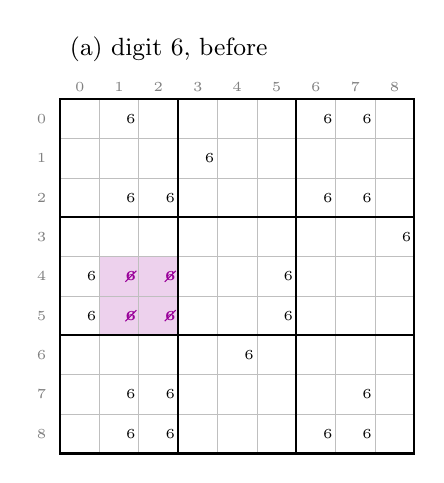
\begin{tikzpicture}[x=1cm,y=1cm]
\node[anchor=south west,font=\small] at (0,4.850) {(a) digit 6, before};
\node[font=\tiny,text=black,inner sep=0] at (0.900,4.250) {6};
\node[font=\tiny,text=black,inner sep=0] at (3.400,4.250) {6};
\node[font=\tiny,text=black,inner sep=0] at (3.900,4.250) {6};
\node[font=\tiny,text=black,inner sep=0] at (1.900,3.750) {6};
\node[font=\tiny,text=black,inner sep=0] at (0.900,3.250) {6};
\node[font=\tiny,text=black,inner sep=0] at (1.400,3.250) {6};
\node[font=\tiny,text=black,inner sep=0] at (3.400,3.250) {6};
\node[font=\tiny,text=black,inner sep=0] at (3.900,3.250) {6};
\node[font=\tiny,text=black,inner sep=0] at (4.400,2.750) {6};
\node[font=\tiny,text=black,inner sep=0] at (0.400,2.250) {6};
\fill[violet!80!magenta!18] (0.500,2.000) rectangle (1.000,2.500);
\node[font=\tiny\bfseries,text=violet!80!magenta,inner sep=0] at (0.900,2.250) {6};
\draw[violet!80!magenta,thin] (0.830,2.180) -- (0.970,2.320);
\fill[violet!80!magenta!18] (1.000,2.000) rectangle (1.500,2.500);
\node[font=\tiny\bfseries,text=violet!80!magenta,inner sep=0] at (1.400,2.250) {6};
\draw[violet!80!magenta,thin] (1.330,2.180) -- (1.470,2.320);
\node[font=\tiny,text=black,inner sep=0] at (2.900,2.250) {6};
\node[font=\tiny,text=black,inner sep=0] at (0.400,1.750) {6};
\fill[violet!80!magenta!18] (0.500,1.500) rectangle (1.000,2.000);
\node[font=\tiny\bfseries,text=violet!80!magenta,inner sep=0] at (0.900,1.750) {6};
\draw[violet!80!magenta,thin] (0.830,1.680) -- (0.970,1.820);
\fill[violet!80!magenta!18] (1.000,1.500) rectangle (1.500,2.000);
\node[font=\tiny\bfseries,text=violet!80!magenta,inner sep=0] at (1.400,1.750) {6};
\draw[violet!80!magenta,thin] (1.330,1.680) -- (1.470,1.820);
\node[font=\tiny,text=black,inner sep=0] at (2.900,1.750) {6};
\node[font=\tiny,text=black,inner sep=0] at (2.400,1.250) {6};
\node[font=\tiny,text=black,inner sep=0] at (0.900,0.750) {6};
\node[font=\tiny,text=black,inner sep=0] at (1.400,0.750) {6};
\node[font=\tiny,text=black,inner sep=0] at (3.900,0.750) {6};
\node[font=\tiny,text=black,inner sep=0] at (0.900,0.250) {6};
\node[font=\tiny,text=black,inner sep=0] at (1.400,0.250) {6};
\node[font=\tiny,text=black,inner sep=0] at (3.400,0.250) {6};
\node[font=\tiny,text=black,inner sep=0] at (3.900,0.250) {6};
\draw[step=0.5,gray!50,very thin] (0,0) grid (4.500,4.500);
\draw[thick] (1.500,0) -- (1.500,4.500);
\draw[thick] (3.000,0) -- (3.000,4.500);
\draw[thick] (0,3.000) -- (4.500,3.000);
\draw[thick] (0,1.500) -- (4.500,1.500);
\draw[thick] (0,0) rectangle (4.500,4.500);
\node[font=\tiny,text=gray] at (0.250,4.650) {0};
\node[font=\tiny,text=gray] at (0.750,4.650) {1};
\node[font=\tiny,text=gray] at (1.250,4.650) {2};
\node[font=\tiny,text=gray] at (1.750,4.650) {3};
\node[font=\tiny,text=gray] at (2.250,4.650) {4};
\node[font=\tiny,text=gray] at (2.750,4.650) {5};
\node[font=\tiny,text=gray] at (3.250,4.650) {6};
\node[font=\tiny,text=gray] at (3.750,4.650) {7};
\node[font=\tiny,text=gray] at (4.250,4.650) {8};
\node[font=\tiny,text=gray,anchor=east] at (-0.05,4.250) {0};
\node[font=\tiny,text=gray,anchor=east] at (-0.05,3.750) {1};
\node[font=\tiny,text=gray,anchor=east] at (-0.05,3.250) {2};
\node[font=\tiny,text=gray,anchor=east] at (-0.05,2.750) {3};
\node[font=\tiny,text=gray,anchor=east] at (-0.05,2.250) {4};
\node[font=\tiny,text=gray,anchor=east] at (-0.05,1.750) {5};
\node[font=\tiny,text=gray,anchor=east] at (-0.05,1.250) {6};
\node[font=\tiny,text=gray,anchor=east] at (-0.05,0.750) {7};
\node[font=\tiny,text=gray,anchor=east] at (-0.05,0.250) {8};
\end{tikzpicture}
\hspace{1cm}
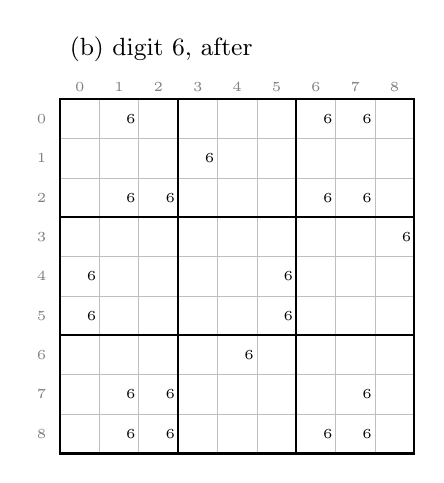
\begin{tikzpicture}[x=1cm,y=1cm]
\node[anchor=south west,font=\small] at (0,4.850) {(b) digit 6, after};
\node[font=\tiny,text=black,inner sep=0] at (0.900,4.250) {6};
\node[font=\tiny,text=black,inner sep=0] at (3.400,4.250) {6};
\node[font=\tiny,text=black,inner sep=0] at (3.900,4.250) {6};
\node[font=\tiny,text=black,inner sep=0] at (1.900,3.750) {6};
\node[font=\tiny,text=black,inner sep=0] at (0.900,3.250) {6};
\node[font=\tiny,text=black,inner sep=0] at (1.400,3.250) {6};
\node[font=\tiny,text=black,inner sep=0] at (3.400,3.250) {6};
\node[font=\tiny,text=black,inner sep=0] at (3.900,3.250) {6};
\node[font=\tiny,text=black,inner sep=0] at (4.400,2.750) {6};
\node[font=\tiny,text=black,inner sep=0] at (0.400,2.250) {6};
\node[font=\tiny,text=black,inner sep=0] at (2.900,2.250) {6};
\node[font=\tiny,text=black,inner sep=0] at (0.400,1.750) {6};
\node[font=\tiny,text=black,inner sep=0] at (2.900,1.750) {6};
\node[font=\tiny,text=black,inner sep=0] at (2.400,1.250) {6};
\node[font=\tiny,text=black,inner sep=0] at (0.900,0.750) {6};
\node[font=\tiny,text=black,inner sep=0] at (1.400,0.750) {6};
\node[font=\tiny,text=black,inner sep=0] at (3.900,0.750) {6};
\node[font=\tiny,text=black,inner sep=0] at (0.900,0.250) {6};
\node[font=\tiny,text=black,inner sep=0] at (1.400,0.250) {6};
\node[font=\tiny,text=black,inner sep=0] at (3.400,0.250) {6};
\node[font=\tiny,text=black,inner sep=0] at (3.900,0.250) {6};
\draw[step=0.5,gray!50,very thin] (0,0) grid (4.500,4.500);
\draw[thick] (1.500,0) -- (1.500,4.500);
\draw[thick] (3.000,0) -- (3.000,4.500);
\draw[thick] (0,3.000) -- (4.500,3.000);
\draw[thick] (0,1.500) -- (4.500,1.500);
\draw[thick] (0,0) rectangle (4.500,4.500);
\node[font=\tiny,text=gray] at (0.250,4.650) {0};
\node[font=\tiny,text=gray] at (0.750,4.650) {1};
\node[font=\tiny,text=gray] at (1.250,4.650) {2};
\node[font=\tiny,text=gray] at (1.750,4.650) {3};
\node[font=\tiny,text=gray] at (2.250,4.650) {4};
\node[font=\tiny,text=gray] at (2.750,4.650) {5};
\node[font=\tiny,text=gray] at (3.250,4.650) {6};
\node[font=\tiny,text=gray] at (3.750,4.650) {7};
\node[font=\tiny,text=gray] at (4.250,4.650) {8};
\node[font=\tiny,text=gray,anchor=east] at (-0.05,4.250) {0};
\node[font=\tiny,text=gray,anchor=east] at (-0.05,3.750) {1};
\node[font=\tiny,text=gray,anchor=east] at (-0.05,3.250) {2};
\node[font=\tiny,text=gray,anchor=east] at (-0.05,2.750) {3};
\node[font=\tiny,text=gray,anchor=east] at (-0.05,2.250) {4};
\node[font=\tiny,text=gray,anchor=east] at (-0.05,1.750) {5};
\node[font=\tiny,text=gray,anchor=east] at (-0.05,1.250) {6};
\node[font=\tiny,text=gray,anchor=east] at (-0.05,0.750) {7};
\node[font=\tiny,text=gray,anchor=east] at (-0.05,0.250) {8};
\end{tikzpicture}
\\[0.5cm]
{\small (c) the tables $B^{6,s}$ (bands $\times$ columns) for stacks 0, 1, 2, before}\\[3pt]
$\begin{array}{c|ccc} & 0 & 1 & 2 \\ \hline \text{band }0 & 0 & \mathbf{1} & \mathbf{1} \\ \text{band }1 & \mathbf{1} & \textcolor{violet!80!magenta}{\mathbf{1}} & \textcolor{violet!80!magenta}{\mathbf{1}} \\ \text{band }2 & 0 & \mathbf{1} & \mathbf{1}\end{array}$\quad$\begin{array}{c|ccc} & 3 & 4 & 5 \\ \hline \text{band }0 & \mathbf{1} & 0 & 0 \\ \text{band }1 & 0 & 0 & \mathbf{1} \\ \text{band }2 & 0 & \mathbf{1} & 0\end{array}$\quad$\begin{array}{c|ccc} & 6 & 7 & 8 \\ \hline \text{band }0 & \mathbf{1} & \mathbf{1} & 0 \\ \text{band }1 & 0 & 0 & \mathbf{1} \\ \text{band }2 & \mathbf{1} & \mathbf{1} & 0\end{array}$
\caption{\textsc{StackRule} (\cref{alg:stack}) for digit 6, the call made inside the band update of \cref{fig:alg-band}. (a), (b): digit 6's candidates over the whole grid; the violet ones are removed. (c): for each stack, a 1 where the band still has digit 6 in that column; entries on some perfect matching are bold, and violet entries are on none. In stack 0, bands 0 and 2 can only use columns 1 and 2, so between them they take both, and band 1 must use the remaining column: it loses columns 1 and 2. That removes 6 from 4 cells. In stacks 1 and 2 every entry is on a perfect matching, so nothing changes there.}
\label{fig:alg-stack}
\end{figure}


% ----------------------------------------------------------------
% removed: % generated by make_figs.py from a real FastBandSolver run; do not edit by hand
\begin{figure}[p]
\centering
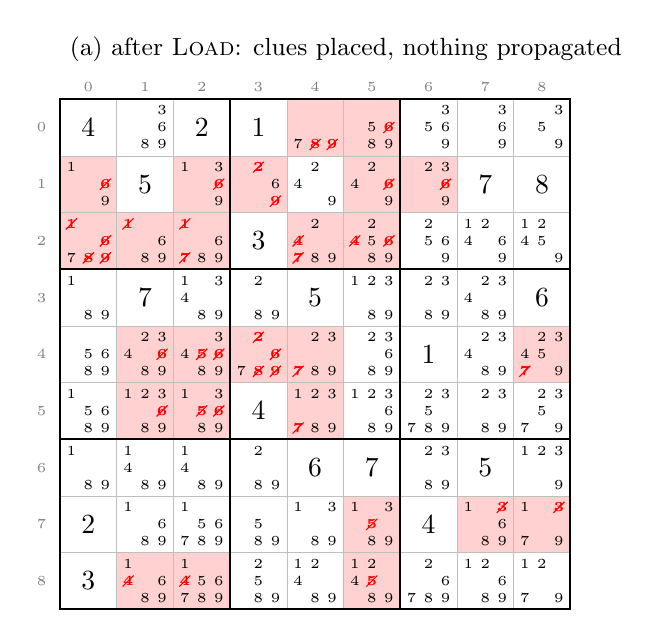
\begin{tikzpicture}[x=1cm,y=1cm]
\node[anchor=south west,font=\small] at (0,6.830) {(a) after \textsc{Load}: clues placed, nothing propagated};
\node[font=\normalsize,text=black] at (0.360,6.120) {4};
\node[font=\tiny,text=black,inner sep=0] at (1.296,6.336) {3};
\node[font=\tiny,text=black,inner sep=0] at (1.296,6.120) {6};
\node[font=\tiny,text=black,inner sep=0] at (1.080,5.904) {8};
\node[font=\tiny,text=black,inner sep=0] at (1.296,5.904) {9};
\node[font=\normalsize,text=black] at (1.800,6.120) {2};
\node[font=\normalsize,text=black] at (2.520,6.120) {1};
\fill[red!18] (2.880,5.760) rectangle (3.600,6.480);
\node[font=\tiny,text=black,inner sep=0] at (3.024,5.904) {7};
\node[font=\tiny\bfseries,text=red,inner sep=0] at (3.240,5.904) {8};
\draw[red,thin] (3.170,5.834) -- (3.310,5.974);
\node[font=\tiny\bfseries,text=red,inner sep=0] at (3.456,5.904) {9};
\draw[red,thin] (3.386,5.834) -- (3.526,5.974);
\fill[red!18] (3.600,5.760) rectangle (4.320,6.480);
\node[font=\tiny,text=black,inner sep=0] at (3.960,6.120) {5};
\node[font=\tiny\bfseries,text=red,inner sep=0] at (4.176,6.120) {6};
\draw[red,thin] (4.106,6.050) -- (4.246,6.190);
\node[font=\tiny,text=black,inner sep=0] at (3.960,5.904) {8};
\node[font=\tiny,text=black,inner sep=0] at (4.176,5.904) {9};
\node[font=\tiny,text=black,inner sep=0] at (4.896,6.336) {3};
\node[font=\tiny,text=black,inner sep=0] at (4.680,6.120) {5};
\node[font=\tiny,text=black,inner sep=0] at (4.896,6.120) {6};
\node[font=\tiny,text=black,inner sep=0] at (4.896,5.904) {9};
\node[font=\tiny,text=black,inner sep=0] at (5.616,6.336) {3};
\node[font=\tiny,text=black,inner sep=0] at (5.616,6.120) {6};
\node[font=\tiny,text=black,inner sep=0] at (5.616,5.904) {9};
\node[font=\tiny,text=black,inner sep=0] at (6.336,6.336) {3};
\node[font=\tiny,text=black,inner sep=0] at (6.120,6.120) {5};
\node[font=\tiny,text=black,inner sep=0] at (6.336,5.904) {9};
\fill[red!18] (0.000,5.040) rectangle (0.720,5.760);
\node[font=\tiny,text=black,inner sep=0] at (0.144,5.616) {1};
\node[font=\tiny\bfseries,text=red,inner sep=0] at (0.576,5.400) {6};
\draw[red,thin] (0.506,5.330) -- (0.646,5.470);
\node[font=\tiny,text=black,inner sep=0] at (0.576,5.184) {9};
\node[font=\normalsize,text=black] at (1.080,5.400) {5};
\fill[red!18] (1.440,5.040) rectangle (2.160,5.760);
\node[font=\tiny,text=black,inner sep=0] at (1.584,5.616) {1};
\node[font=\tiny,text=black,inner sep=0] at (2.016,5.616) {3};
\node[font=\tiny\bfseries,text=red,inner sep=0] at (2.016,5.400) {6};
\draw[red,thin] (1.946,5.330) -- (2.086,5.470);
\node[font=\tiny,text=black,inner sep=0] at (2.016,5.184) {9};
\fill[red!18] (2.160,5.040) rectangle (2.880,5.760);
\node[font=\tiny\bfseries,text=red,inner sep=0] at (2.520,5.616) {2};
\draw[red,thin] (2.450,5.546) -- (2.590,5.686);
\node[font=\tiny,text=black,inner sep=0] at (2.736,5.400) {6};
\node[font=\tiny\bfseries,text=red,inner sep=0] at (2.736,5.184) {9};
\draw[red,thin] (2.666,5.114) -- (2.806,5.254);
\node[font=\tiny,text=black,inner sep=0] at (3.240,5.616) {2};
\node[font=\tiny,text=black,inner sep=0] at (3.024,5.400) {4};
\node[font=\tiny,text=black,inner sep=0] at (3.456,5.184) {9};
\fill[red!18] (3.600,5.040) rectangle (4.320,5.760);
\node[font=\tiny,text=black,inner sep=0] at (3.960,5.616) {2};
\node[font=\tiny,text=black,inner sep=0] at (3.744,5.400) {4};
\node[font=\tiny\bfseries,text=red,inner sep=0] at (4.176,5.400) {6};
\draw[red,thin] (4.106,5.330) -- (4.246,5.470);
\node[font=\tiny,text=black,inner sep=0] at (4.176,5.184) {9};
\fill[red!18] (4.320,5.040) rectangle (5.040,5.760);
\node[font=\tiny,text=black,inner sep=0] at (4.680,5.616) {2};
\node[font=\tiny,text=black,inner sep=0] at (4.896,5.616) {3};
\node[font=\tiny\bfseries,text=red,inner sep=0] at (4.896,5.400) {6};
\draw[red,thin] (4.826,5.330) -- (4.966,5.470);
\node[font=\tiny,text=black,inner sep=0] at (4.896,5.184) {9};
\node[font=\normalsize,text=black] at (5.400,5.400) {7};
\node[font=\normalsize,text=black] at (6.120,5.400) {8};
\fill[red!18] (0.000,4.320) rectangle (0.720,5.040);
\node[font=\tiny\bfseries,text=red,inner sep=0] at (0.144,4.896) {1};
\draw[red,thin] (0.074,4.826) -- (0.214,4.966);
\node[font=\tiny\bfseries,text=red,inner sep=0] at (0.576,4.680) {6};
\draw[red,thin] (0.506,4.610) -- (0.646,4.750);
\node[font=\tiny,text=black,inner sep=0] at (0.144,4.464) {7};
\node[font=\tiny\bfseries,text=red,inner sep=0] at (0.360,4.464) {8};
\draw[red,thin] (0.290,4.394) -- (0.430,4.534);
\node[font=\tiny\bfseries,text=red,inner sep=0] at (0.576,4.464) {9};
\draw[red,thin] (0.506,4.394) -- (0.646,4.534);
\fill[red!18] (0.720,4.320) rectangle (1.440,5.040);
\node[font=\tiny\bfseries,text=red,inner sep=0] at (0.864,4.896) {1};
\draw[red,thin] (0.794,4.826) -- (0.934,4.966);
\node[font=\tiny,text=black,inner sep=0] at (1.296,4.680) {6};
\node[font=\tiny,text=black,inner sep=0] at (1.080,4.464) {8};
\node[font=\tiny,text=black,inner sep=0] at (1.296,4.464) {9};
\fill[red!18] (1.440,4.320) rectangle (2.160,5.040);
\node[font=\tiny\bfseries,text=red,inner sep=0] at (1.584,4.896) {1};
\draw[red,thin] (1.514,4.826) -- (1.654,4.966);
\node[font=\tiny,text=black,inner sep=0] at (2.016,4.680) {6};
\node[font=\tiny\bfseries,text=red,inner sep=0] at (1.584,4.464) {7};
\draw[red,thin] (1.514,4.394) -- (1.654,4.534);
\node[font=\tiny,text=black,inner sep=0] at (1.800,4.464) {8};
\node[font=\tiny,text=black,inner sep=0] at (2.016,4.464) {9};
\node[font=\normalsize,text=black] at (2.520,4.680) {3};
\fill[red!18] (2.880,4.320) rectangle (3.600,5.040);
\node[font=\tiny,text=black,inner sep=0] at (3.240,4.896) {2};
\node[font=\tiny\bfseries,text=red,inner sep=0] at (3.024,4.680) {4};
\draw[red,thin] (2.954,4.610) -- (3.094,4.750);
\node[font=\tiny\bfseries,text=red,inner sep=0] at (3.024,4.464) {7};
\draw[red,thin] (2.954,4.394) -- (3.094,4.534);
\node[font=\tiny,text=black,inner sep=0] at (3.240,4.464) {8};
\node[font=\tiny,text=black,inner sep=0] at (3.456,4.464) {9};
\fill[red!18] (3.600,4.320) rectangle (4.320,5.040);
\node[font=\tiny,text=black,inner sep=0] at (3.960,4.896) {2};
\node[font=\tiny\bfseries,text=red,inner sep=0] at (3.744,4.680) {4};
\draw[red,thin] (3.674,4.610) -- (3.814,4.750);
\node[font=\tiny,text=black,inner sep=0] at (3.960,4.680) {5};
\node[font=\tiny\bfseries,text=red,inner sep=0] at (4.176,4.680) {6};
\draw[red,thin] (4.106,4.610) -- (4.246,4.750);
\node[font=\tiny,text=black,inner sep=0] at (3.960,4.464) {8};
\node[font=\tiny,text=black,inner sep=0] at (4.176,4.464) {9};
\node[font=\tiny,text=black,inner sep=0] at (4.680,4.896) {2};
\node[font=\tiny,text=black,inner sep=0] at (4.680,4.680) {5};
\node[font=\tiny,text=black,inner sep=0] at (4.896,4.680) {6};
\node[font=\tiny,text=black,inner sep=0] at (4.896,4.464) {9};
\node[font=\tiny,text=black,inner sep=0] at (5.184,4.896) {1};
\node[font=\tiny,text=black,inner sep=0] at (5.400,4.896) {2};
\node[font=\tiny,text=black,inner sep=0] at (5.184,4.680) {4};
\node[font=\tiny,text=black,inner sep=0] at (5.616,4.680) {6};
\node[font=\tiny,text=black,inner sep=0] at (5.616,4.464) {9};
\node[font=\tiny,text=black,inner sep=0] at (5.904,4.896) {1};
\node[font=\tiny,text=black,inner sep=0] at (6.120,4.896) {2};
\node[font=\tiny,text=black,inner sep=0] at (5.904,4.680) {4};
\node[font=\tiny,text=black,inner sep=0] at (6.120,4.680) {5};
\node[font=\tiny,text=black,inner sep=0] at (6.336,4.464) {9};
\node[font=\tiny,text=black,inner sep=0] at (0.144,4.176) {1};
\node[font=\tiny,text=black,inner sep=0] at (0.360,3.744) {8};
\node[font=\tiny,text=black,inner sep=0] at (0.576,3.744) {9};
\node[font=\normalsize,text=black] at (1.080,3.960) {7};
\node[font=\tiny,text=black,inner sep=0] at (1.584,4.176) {1};
\node[font=\tiny,text=black,inner sep=0] at (2.016,4.176) {3};
\node[font=\tiny,text=black,inner sep=0] at (1.584,3.960) {4};
\node[font=\tiny,text=black,inner sep=0] at (1.800,3.744) {8};
\node[font=\tiny,text=black,inner sep=0] at (2.016,3.744) {9};
\node[font=\tiny,text=black,inner sep=0] at (2.520,4.176) {2};
\node[font=\tiny,text=black,inner sep=0] at (2.520,3.744) {8};
\node[font=\tiny,text=black,inner sep=0] at (2.736,3.744) {9};
\node[font=\normalsize,text=black] at (3.240,3.960) {5};
\node[font=\tiny,text=black,inner sep=0] at (3.744,4.176) {1};
\node[font=\tiny,text=black,inner sep=0] at (3.960,4.176) {2};
\node[font=\tiny,text=black,inner sep=0] at (4.176,4.176) {3};
\node[font=\tiny,text=black,inner sep=0] at (3.960,3.744) {8};
\node[font=\tiny,text=black,inner sep=0] at (4.176,3.744) {9};
\node[font=\tiny,text=black,inner sep=0] at (4.680,4.176) {2};
\node[font=\tiny,text=black,inner sep=0] at (4.896,4.176) {3};
\node[font=\tiny,text=black,inner sep=0] at (4.680,3.744) {8};
\node[font=\tiny,text=black,inner sep=0] at (4.896,3.744) {9};
\node[font=\tiny,text=black,inner sep=0] at (5.400,4.176) {2};
\node[font=\tiny,text=black,inner sep=0] at (5.616,4.176) {3};
\node[font=\tiny,text=black,inner sep=0] at (5.184,3.960) {4};
\node[font=\tiny,text=black,inner sep=0] at (5.400,3.744) {8};
\node[font=\tiny,text=black,inner sep=0] at (5.616,3.744) {9};
\node[font=\normalsize,text=black] at (6.120,3.960) {6};
\node[font=\tiny,text=black,inner sep=0] at (0.360,3.240) {5};
\node[font=\tiny,text=black,inner sep=0] at (0.576,3.240) {6};
\node[font=\tiny,text=black,inner sep=0] at (0.360,3.024) {8};
\node[font=\tiny,text=black,inner sep=0] at (0.576,3.024) {9};
\fill[red!18] (0.720,2.880) rectangle (1.440,3.600);
\node[font=\tiny,text=black,inner sep=0] at (1.080,3.456) {2};
\node[font=\tiny,text=black,inner sep=0] at (1.296,3.456) {3};
\node[font=\tiny,text=black,inner sep=0] at (0.864,3.240) {4};
\node[font=\tiny\bfseries,text=red,inner sep=0] at (1.296,3.240) {6};
\draw[red,thin] (1.226,3.170) -- (1.366,3.310);
\node[font=\tiny,text=black,inner sep=0] at (1.080,3.024) {8};
\node[font=\tiny,text=black,inner sep=0] at (1.296,3.024) {9};
\fill[red!18] (1.440,2.880) rectangle (2.160,3.600);
\node[font=\tiny,text=black,inner sep=0] at (2.016,3.456) {3};
\node[font=\tiny,text=black,inner sep=0] at (1.584,3.240) {4};
\node[font=\tiny\bfseries,text=red,inner sep=0] at (1.800,3.240) {5};
\draw[red,thin] (1.730,3.170) -- (1.870,3.310);
\node[font=\tiny\bfseries,text=red,inner sep=0] at (2.016,3.240) {6};
\draw[red,thin] (1.946,3.170) -- (2.086,3.310);
\node[font=\tiny,text=black,inner sep=0] at (1.800,3.024) {8};
\node[font=\tiny,text=black,inner sep=0] at (2.016,3.024) {9};
\fill[red!18] (2.160,2.880) rectangle (2.880,3.600);
\node[font=\tiny\bfseries,text=red,inner sep=0] at (2.520,3.456) {2};
\draw[red,thin] (2.450,3.386) -- (2.590,3.526);
\node[font=\tiny\bfseries,text=red,inner sep=0] at (2.736,3.240) {6};
\draw[red,thin] (2.666,3.170) -- (2.806,3.310);
\node[font=\tiny,text=black,inner sep=0] at (2.304,3.024) {7};
\node[font=\tiny\bfseries,text=red,inner sep=0] at (2.520,3.024) {8};
\draw[red,thin] (2.450,2.954) -- (2.590,3.094);
\node[font=\tiny\bfseries,text=red,inner sep=0] at (2.736,3.024) {9};
\draw[red,thin] (2.666,2.954) -- (2.806,3.094);
\fill[red!18] (2.880,2.880) rectangle (3.600,3.600);
\node[font=\tiny,text=black,inner sep=0] at (3.240,3.456) {2};
\node[font=\tiny,text=black,inner sep=0] at (3.456,3.456) {3};
\node[font=\tiny\bfseries,text=red,inner sep=0] at (3.024,3.024) {7};
\draw[red,thin] (2.954,2.954) -- (3.094,3.094);
\node[font=\tiny,text=black,inner sep=0] at (3.240,3.024) {8};
\node[font=\tiny,text=black,inner sep=0] at (3.456,3.024) {9};
\node[font=\tiny,text=black,inner sep=0] at (3.960,3.456) {2};
\node[font=\tiny,text=black,inner sep=0] at (4.176,3.456) {3};
\node[font=\tiny,text=black,inner sep=0] at (4.176,3.240) {6};
\node[font=\tiny,text=black,inner sep=0] at (3.960,3.024) {8};
\node[font=\tiny,text=black,inner sep=0] at (4.176,3.024) {9};
\node[font=\normalsize,text=black] at (4.680,3.240) {1};
\node[font=\tiny,text=black,inner sep=0] at (5.400,3.456) {2};
\node[font=\tiny,text=black,inner sep=0] at (5.616,3.456) {3};
\node[font=\tiny,text=black,inner sep=0] at (5.184,3.240) {4};
\node[font=\tiny,text=black,inner sep=0] at (5.400,3.024) {8};
\node[font=\tiny,text=black,inner sep=0] at (5.616,3.024) {9};
\fill[red!18] (5.760,2.880) rectangle (6.480,3.600);
\node[font=\tiny,text=black,inner sep=0] at (6.120,3.456) {2};
\node[font=\tiny,text=black,inner sep=0] at (6.336,3.456) {3};
\node[font=\tiny,text=black,inner sep=0] at (5.904,3.240) {4};
\node[font=\tiny,text=black,inner sep=0] at (6.120,3.240) {5};
\node[font=\tiny\bfseries,text=red,inner sep=0] at (5.904,3.024) {7};
\draw[red,thin] (5.834,2.954) -- (5.974,3.094);
\node[font=\tiny,text=black,inner sep=0] at (6.336,3.024) {9};
\node[font=\tiny,text=black,inner sep=0] at (0.144,2.736) {1};
\node[font=\tiny,text=black,inner sep=0] at (0.360,2.520) {5};
\node[font=\tiny,text=black,inner sep=0] at (0.576,2.520) {6};
\node[font=\tiny,text=black,inner sep=0] at (0.360,2.304) {8};
\node[font=\tiny,text=black,inner sep=0] at (0.576,2.304) {9};
\fill[red!18] (0.720,2.160) rectangle (1.440,2.880);
\node[font=\tiny,text=black,inner sep=0] at (0.864,2.736) {1};
\node[font=\tiny,text=black,inner sep=0] at (1.080,2.736) {2};
\node[font=\tiny,text=black,inner sep=0] at (1.296,2.736) {3};
\node[font=\tiny\bfseries,text=red,inner sep=0] at (1.296,2.520) {6};
\draw[red,thin] (1.226,2.450) -- (1.366,2.590);
\node[font=\tiny,text=black,inner sep=0] at (1.080,2.304) {8};
\node[font=\tiny,text=black,inner sep=0] at (1.296,2.304) {9};
\fill[red!18] (1.440,2.160) rectangle (2.160,2.880);
\node[font=\tiny,text=black,inner sep=0] at (1.584,2.736) {1};
\node[font=\tiny,text=black,inner sep=0] at (2.016,2.736) {3};
\node[font=\tiny\bfseries,text=red,inner sep=0] at (1.800,2.520) {5};
\draw[red,thin] (1.730,2.450) -- (1.870,2.590);
\node[font=\tiny\bfseries,text=red,inner sep=0] at (2.016,2.520) {6};
\draw[red,thin] (1.946,2.450) -- (2.086,2.590);
\node[font=\tiny,text=black,inner sep=0] at (1.800,2.304) {8};
\node[font=\tiny,text=black,inner sep=0] at (2.016,2.304) {9};
\node[font=\normalsize,text=black] at (2.520,2.520) {4};
\fill[red!18] (2.880,2.160) rectangle (3.600,2.880);
\node[font=\tiny,text=black,inner sep=0] at (3.024,2.736) {1};
\node[font=\tiny,text=black,inner sep=0] at (3.240,2.736) {2};
\node[font=\tiny,text=black,inner sep=0] at (3.456,2.736) {3};
\node[font=\tiny\bfseries,text=red,inner sep=0] at (3.024,2.304) {7};
\draw[red,thin] (2.954,2.234) -- (3.094,2.374);
\node[font=\tiny,text=black,inner sep=0] at (3.240,2.304) {8};
\node[font=\tiny,text=black,inner sep=0] at (3.456,2.304) {9};
\node[font=\tiny,text=black,inner sep=0] at (3.744,2.736) {1};
\node[font=\tiny,text=black,inner sep=0] at (3.960,2.736) {2};
\node[font=\tiny,text=black,inner sep=0] at (4.176,2.736) {3};
\node[font=\tiny,text=black,inner sep=0] at (4.176,2.520) {6};
\node[font=\tiny,text=black,inner sep=0] at (3.960,2.304) {8};
\node[font=\tiny,text=black,inner sep=0] at (4.176,2.304) {9};
\node[font=\tiny,text=black,inner sep=0] at (4.680,2.736) {2};
\node[font=\tiny,text=black,inner sep=0] at (4.896,2.736) {3};
\node[font=\tiny,text=black,inner sep=0] at (4.680,2.520) {5};
\node[font=\tiny,text=black,inner sep=0] at (4.464,2.304) {7};
\node[font=\tiny,text=black,inner sep=0] at (4.680,2.304) {8};
\node[font=\tiny,text=black,inner sep=0] at (4.896,2.304) {9};
\node[font=\tiny,text=black,inner sep=0] at (5.400,2.736) {2};
\node[font=\tiny,text=black,inner sep=0] at (5.616,2.736) {3};
\node[font=\tiny,text=black,inner sep=0] at (5.400,2.304) {8};
\node[font=\tiny,text=black,inner sep=0] at (5.616,2.304) {9};
\node[font=\tiny,text=black,inner sep=0] at (6.120,2.736) {2};
\node[font=\tiny,text=black,inner sep=0] at (6.336,2.736) {3};
\node[font=\tiny,text=black,inner sep=0] at (6.120,2.520) {5};
\node[font=\tiny,text=black,inner sep=0] at (5.904,2.304) {7};
\node[font=\tiny,text=black,inner sep=0] at (6.336,2.304) {9};
\node[font=\tiny,text=black,inner sep=0] at (0.144,2.016) {1};
\node[font=\tiny,text=black,inner sep=0] at (0.360,1.584) {8};
\node[font=\tiny,text=black,inner sep=0] at (0.576,1.584) {9};
\node[font=\tiny,text=black,inner sep=0] at (0.864,2.016) {1};
\node[font=\tiny,text=black,inner sep=0] at (0.864,1.800) {4};
\node[font=\tiny,text=black,inner sep=0] at (1.080,1.584) {8};
\node[font=\tiny,text=black,inner sep=0] at (1.296,1.584) {9};
\node[font=\tiny,text=black,inner sep=0] at (1.584,2.016) {1};
\node[font=\tiny,text=black,inner sep=0] at (1.584,1.800) {4};
\node[font=\tiny,text=black,inner sep=0] at (1.800,1.584) {8};
\node[font=\tiny,text=black,inner sep=0] at (2.016,1.584) {9};
\node[font=\tiny,text=black,inner sep=0] at (2.520,2.016) {2};
\node[font=\tiny,text=black,inner sep=0] at (2.520,1.584) {8};
\node[font=\tiny,text=black,inner sep=0] at (2.736,1.584) {9};
\node[font=\normalsize,text=black] at (3.240,1.800) {6};
\node[font=\normalsize,text=black] at (3.960,1.800) {7};
\node[font=\tiny,text=black,inner sep=0] at (4.680,2.016) {2};
\node[font=\tiny,text=black,inner sep=0] at (4.896,2.016) {3};
\node[font=\tiny,text=black,inner sep=0] at (4.680,1.584) {8};
\node[font=\tiny,text=black,inner sep=0] at (4.896,1.584) {9};
\node[font=\normalsize,text=black] at (5.400,1.800) {5};
\node[font=\tiny,text=black,inner sep=0] at (5.904,2.016) {1};
\node[font=\tiny,text=black,inner sep=0] at (6.120,2.016) {2};
\node[font=\tiny,text=black,inner sep=0] at (6.336,2.016) {3};
\node[font=\tiny,text=black,inner sep=0] at (6.336,1.584) {9};
\node[font=\normalsize,text=black] at (0.360,1.080) {2};
\node[font=\tiny,text=black,inner sep=0] at (0.864,1.296) {1};
\node[font=\tiny,text=black,inner sep=0] at (1.296,1.080) {6};
\node[font=\tiny,text=black,inner sep=0] at (1.080,0.864) {8};
\node[font=\tiny,text=black,inner sep=0] at (1.296,0.864) {9};
\node[font=\tiny,text=black,inner sep=0] at (1.584,1.296) {1};
\node[font=\tiny,text=black,inner sep=0] at (1.800,1.080) {5};
\node[font=\tiny,text=black,inner sep=0] at (2.016,1.080) {6};
\node[font=\tiny,text=black,inner sep=0] at (1.584,0.864) {7};
\node[font=\tiny,text=black,inner sep=0] at (1.800,0.864) {8};
\node[font=\tiny,text=black,inner sep=0] at (2.016,0.864) {9};
\node[font=\tiny,text=black,inner sep=0] at (2.520,1.080) {5};
\node[font=\tiny,text=black,inner sep=0] at (2.520,0.864) {8};
\node[font=\tiny,text=black,inner sep=0] at (2.736,0.864) {9};
\node[font=\tiny,text=black,inner sep=0] at (3.024,1.296) {1};
\node[font=\tiny,text=black,inner sep=0] at (3.456,1.296) {3};
\node[font=\tiny,text=black,inner sep=0] at (3.240,0.864) {8};
\node[font=\tiny,text=black,inner sep=0] at (3.456,0.864) {9};
\fill[red!18] (3.600,0.720) rectangle (4.320,1.440);
\node[font=\tiny,text=black,inner sep=0] at (3.744,1.296) {1};
\node[font=\tiny,text=black,inner sep=0] at (4.176,1.296) {3};
\node[font=\tiny\bfseries,text=red,inner sep=0] at (3.960,1.080) {5};
\draw[red,thin] (3.890,1.010) -- (4.030,1.150);
\node[font=\tiny,text=black,inner sep=0] at (3.960,0.864) {8};
\node[font=\tiny,text=black,inner sep=0] at (4.176,0.864) {9};
\node[font=\normalsize,text=black] at (4.680,1.080) {4};
\fill[red!18] (5.040,0.720) rectangle (5.760,1.440);
\node[font=\tiny,text=black,inner sep=0] at (5.184,1.296) {1};
\node[font=\tiny\bfseries,text=red,inner sep=0] at (5.616,1.296) {3};
\draw[red,thin] (5.546,1.226) -- (5.686,1.366);
\node[font=\tiny,text=black,inner sep=0] at (5.616,1.080) {6};
\node[font=\tiny,text=black,inner sep=0] at (5.400,0.864) {8};
\node[font=\tiny,text=black,inner sep=0] at (5.616,0.864) {9};
\fill[red!18] (5.760,0.720) rectangle (6.480,1.440);
\node[font=\tiny,text=black,inner sep=0] at (5.904,1.296) {1};
\node[font=\tiny\bfseries,text=red,inner sep=0] at (6.336,1.296) {3};
\draw[red,thin] (6.266,1.226) -- (6.406,1.366);
\node[font=\tiny,text=black,inner sep=0] at (5.904,0.864) {7};
\node[font=\tiny,text=black,inner sep=0] at (6.336,0.864) {9};
\node[font=\normalsize,text=black] at (0.360,0.360) {3};
\fill[red!18] (0.720,0.000) rectangle (1.440,0.720);
\node[font=\tiny,text=black,inner sep=0] at (0.864,0.576) {1};
\node[font=\tiny\bfseries,text=red,inner sep=0] at (0.864,0.360) {4};
\draw[red,thin] (0.794,0.290) -- (0.934,0.430);
\node[font=\tiny,text=black,inner sep=0] at (1.296,0.360) {6};
\node[font=\tiny,text=black,inner sep=0] at (1.080,0.144) {8};
\node[font=\tiny,text=black,inner sep=0] at (1.296,0.144) {9};
\fill[red!18] (1.440,0.000) rectangle (2.160,0.720);
\node[font=\tiny,text=black,inner sep=0] at (1.584,0.576) {1};
\node[font=\tiny\bfseries,text=red,inner sep=0] at (1.584,0.360) {4};
\draw[red,thin] (1.514,0.290) -- (1.654,0.430);
\node[font=\tiny,text=black,inner sep=0] at (1.800,0.360) {5};
\node[font=\tiny,text=black,inner sep=0] at (2.016,0.360) {6};
\node[font=\tiny,text=black,inner sep=0] at (1.584,0.144) {7};
\node[font=\tiny,text=black,inner sep=0] at (1.800,0.144) {8};
\node[font=\tiny,text=black,inner sep=0] at (2.016,0.144) {9};
\node[font=\tiny,text=black,inner sep=0] at (2.520,0.576) {2};
\node[font=\tiny,text=black,inner sep=0] at (2.520,0.360) {5};
\node[font=\tiny,text=black,inner sep=0] at (2.520,0.144) {8};
\node[font=\tiny,text=black,inner sep=0] at (2.736,0.144) {9};
\node[font=\tiny,text=black,inner sep=0] at (3.024,0.576) {1};
\node[font=\tiny,text=black,inner sep=0] at (3.240,0.576) {2};
\node[font=\tiny,text=black,inner sep=0] at (3.024,0.360) {4};
\node[font=\tiny,text=black,inner sep=0] at (3.240,0.144) {8};
\node[font=\tiny,text=black,inner sep=0] at (3.456,0.144) {9};
\fill[red!18] (3.600,0.000) rectangle (4.320,0.720);
\node[font=\tiny,text=black,inner sep=0] at (3.744,0.576) {1};
\node[font=\tiny,text=black,inner sep=0] at (3.960,0.576) {2};
\node[font=\tiny,text=black,inner sep=0] at (3.744,0.360) {4};
\node[font=\tiny\bfseries,text=red,inner sep=0] at (3.960,0.360) {5};
\draw[red,thin] (3.890,0.290) -- (4.030,0.430);
\node[font=\tiny,text=black,inner sep=0] at (3.960,0.144) {8};
\node[font=\tiny,text=black,inner sep=0] at (4.176,0.144) {9};
\node[font=\tiny,text=black,inner sep=0] at (4.680,0.576) {2};
\node[font=\tiny,text=black,inner sep=0] at (4.896,0.360) {6};
\node[font=\tiny,text=black,inner sep=0] at (4.464,0.144) {7};
\node[font=\tiny,text=black,inner sep=0] at (4.680,0.144) {8};
\node[font=\tiny,text=black,inner sep=0] at (4.896,0.144) {9};
\node[font=\tiny,text=black,inner sep=0] at (5.184,0.576) {1};
\node[font=\tiny,text=black,inner sep=0] at (5.400,0.576) {2};
\node[font=\tiny,text=black,inner sep=0] at (5.616,0.360) {6};
\node[font=\tiny,text=black,inner sep=0] at (5.400,0.144) {8};
\node[font=\tiny,text=black,inner sep=0] at (5.616,0.144) {9};
\node[font=\tiny,text=black,inner sep=0] at (5.904,0.576) {1};
\node[font=\tiny,text=black,inner sep=0] at (6.120,0.576) {2};
\node[font=\tiny,text=black,inner sep=0] at (5.904,0.144) {7};
\node[font=\tiny,text=black,inner sep=0] at (6.336,0.144) {9};
\draw[step=0.72,gray!50,very thin] (0,0) grid (6.480,6.480);
\draw[thick] (2.160,0) -- (2.160,6.480);
\draw[thick] (4.320,0) -- (4.320,6.480);
\draw[thick] (0,4.320) -- (6.480,4.320);
\draw[thick] (0,2.160) -- (6.480,2.160);
\draw[thick] (0,0) rectangle (6.480,6.480);
\node[font=\tiny,text=gray] at (0.360,6.630) {0};
\node[font=\tiny,text=gray] at (1.080,6.630) {1};
\node[font=\tiny,text=gray] at (1.800,6.630) {2};
\node[font=\tiny,text=gray] at (2.520,6.630) {3};
\node[font=\tiny,text=gray] at (3.240,6.630) {4};
\node[font=\tiny,text=gray] at (3.960,6.630) {5};
\node[font=\tiny,text=gray] at (4.680,6.630) {6};
\node[font=\tiny,text=gray] at (5.400,6.630) {7};
\node[font=\tiny,text=gray] at (6.120,6.630) {8};
\node[font=\tiny,text=gray,anchor=east] at (-0.05,6.120) {0};
\node[font=\tiny,text=gray,anchor=east] at (-0.05,5.400) {1};
\node[font=\tiny,text=gray,anchor=east] at (-0.05,4.680) {2};
\node[font=\tiny,text=gray,anchor=east] at (-0.05,3.960) {3};
\node[font=\tiny,text=gray,anchor=east] at (-0.05,3.240) {4};
\node[font=\tiny,text=gray,anchor=east] at (-0.05,2.520) {5};
\node[font=\tiny,text=gray,anchor=east] at (-0.05,1.800) {6};
\node[font=\tiny,text=gray,anchor=east] at (-0.05,1.080) {7};
\node[font=\tiny,text=gray,anchor=east] at (-0.05,0.360) {8};
\end{tikzpicture}
\\[0.4cm]
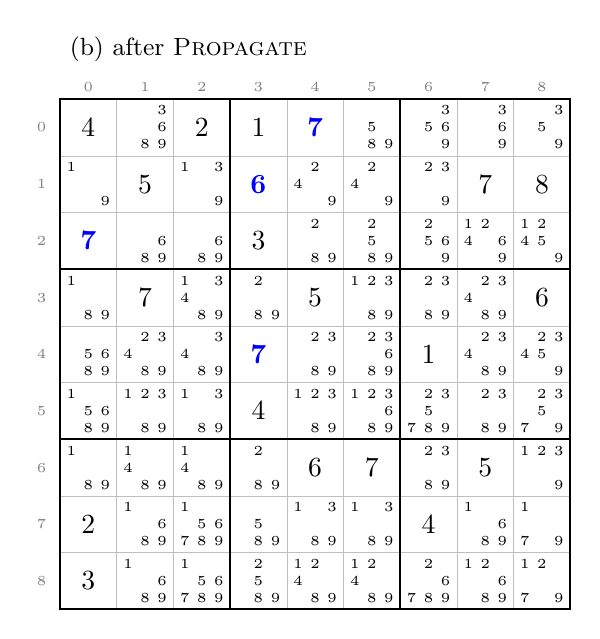
\begin{tikzpicture}[x=1cm,y=1cm]
\node[anchor=south west,font=\small] at (0,6.830) {(b) after \textsc{Propagate}};
\node[font=\normalsize,text=black] at (0.360,6.120) {4};
\node[font=\tiny,text=black,inner sep=0] at (1.296,6.336) {3};
\node[font=\tiny,text=black,inner sep=0] at (1.296,6.120) {6};
\node[font=\tiny,text=black,inner sep=0] at (1.080,5.904) {8};
\node[font=\tiny,text=black,inner sep=0] at (1.296,5.904) {9};
\node[font=\normalsize,text=black] at (1.800,6.120) {2};
\node[font=\normalsize,text=black] at (2.520,6.120) {1};
\node[font=\normalsize\bfseries,text=blue] at (3.240,6.120) {7};
\node[font=\tiny,text=black,inner sep=0] at (3.960,6.120) {5};
\node[font=\tiny,text=black,inner sep=0] at (3.960,5.904) {8};
\node[font=\tiny,text=black,inner sep=0] at (4.176,5.904) {9};
\node[font=\tiny,text=black,inner sep=0] at (4.896,6.336) {3};
\node[font=\tiny,text=black,inner sep=0] at (4.680,6.120) {5};
\node[font=\tiny,text=black,inner sep=0] at (4.896,6.120) {6};
\node[font=\tiny,text=black,inner sep=0] at (4.896,5.904) {9};
\node[font=\tiny,text=black,inner sep=0] at (5.616,6.336) {3};
\node[font=\tiny,text=black,inner sep=0] at (5.616,6.120) {6};
\node[font=\tiny,text=black,inner sep=0] at (5.616,5.904) {9};
\node[font=\tiny,text=black,inner sep=0] at (6.336,6.336) {3};
\node[font=\tiny,text=black,inner sep=0] at (6.120,6.120) {5};
\node[font=\tiny,text=black,inner sep=0] at (6.336,5.904) {9};
\node[font=\tiny,text=black,inner sep=0] at (0.144,5.616) {1};
\node[font=\tiny,text=black,inner sep=0] at (0.576,5.184) {9};
\node[font=\normalsize,text=black] at (1.080,5.400) {5};
\node[font=\tiny,text=black,inner sep=0] at (1.584,5.616) {1};
\node[font=\tiny,text=black,inner sep=0] at (2.016,5.616) {3};
\node[font=\tiny,text=black,inner sep=0] at (2.016,5.184) {9};
\node[font=\normalsize\bfseries,text=blue] at (2.520,5.400) {6};
\node[font=\tiny,text=black,inner sep=0] at (3.240,5.616) {2};
\node[font=\tiny,text=black,inner sep=0] at (3.024,5.400) {4};
\node[font=\tiny,text=black,inner sep=0] at (3.456,5.184) {9};
\node[font=\tiny,text=black,inner sep=0] at (3.960,5.616) {2};
\node[font=\tiny,text=black,inner sep=0] at (3.744,5.400) {4};
\node[font=\tiny,text=black,inner sep=0] at (4.176,5.184) {9};
\node[font=\tiny,text=black,inner sep=0] at (4.680,5.616) {2};
\node[font=\tiny,text=black,inner sep=0] at (4.896,5.616) {3};
\node[font=\tiny,text=black,inner sep=0] at (4.896,5.184) {9};
\node[font=\normalsize,text=black] at (5.400,5.400) {7};
\node[font=\normalsize,text=black] at (6.120,5.400) {8};
\node[font=\normalsize\bfseries,text=blue] at (0.360,4.680) {7};
\node[font=\tiny,text=black,inner sep=0] at (1.296,4.680) {6};
\node[font=\tiny,text=black,inner sep=0] at (1.080,4.464) {8};
\node[font=\tiny,text=black,inner sep=0] at (1.296,4.464) {9};
\node[font=\tiny,text=black,inner sep=0] at (2.016,4.680) {6};
\node[font=\tiny,text=black,inner sep=0] at (1.800,4.464) {8};
\node[font=\tiny,text=black,inner sep=0] at (2.016,4.464) {9};
\node[font=\normalsize,text=black] at (2.520,4.680) {3};
\node[font=\tiny,text=black,inner sep=0] at (3.240,4.896) {2};
\node[font=\tiny,text=black,inner sep=0] at (3.240,4.464) {8};
\node[font=\tiny,text=black,inner sep=0] at (3.456,4.464) {9};
\node[font=\tiny,text=black,inner sep=0] at (3.960,4.896) {2};
\node[font=\tiny,text=black,inner sep=0] at (3.960,4.680) {5};
\node[font=\tiny,text=black,inner sep=0] at (3.960,4.464) {8};
\node[font=\tiny,text=black,inner sep=0] at (4.176,4.464) {9};
\node[font=\tiny,text=black,inner sep=0] at (4.680,4.896) {2};
\node[font=\tiny,text=black,inner sep=0] at (4.680,4.680) {5};
\node[font=\tiny,text=black,inner sep=0] at (4.896,4.680) {6};
\node[font=\tiny,text=black,inner sep=0] at (4.896,4.464) {9};
\node[font=\tiny,text=black,inner sep=0] at (5.184,4.896) {1};
\node[font=\tiny,text=black,inner sep=0] at (5.400,4.896) {2};
\node[font=\tiny,text=black,inner sep=0] at (5.184,4.680) {4};
\node[font=\tiny,text=black,inner sep=0] at (5.616,4.680) {6};
\node[font=\tiny,text=black,inner sep=0] at (5.616,4.464) {9};
\node[font=\tiny,text=black,inner sep=0] at (5.904,4.896) {1};
\node[font=\tiny,text=black,inner sep=0] at (6.120,4.896) {2};
\node[font=\tiny,text=black,inner sep=0] at (5.904,4.680) {4};
\node[font=\tiny,text=black,inner sep=0] at (6.120,4.680) {5};
\node[font=\tiny,text=black,inner sep=0] at (6.336,4.464) {9};
\node[font=\tiny,text=black,inner sep=0] at (0.144,4.176) {1};
\node[font=\tiny,text=black,inner sep=0] at (0.360,3.744) {8};
\node[font=\tiny,text=black,inner sep=0] at (0.576,3.744) {9};
\node[font=\normalsize,text=black] at (1.080,3.960) {7};
\node[font=\tiny,text=black,inner sep=0] at (1.584,4.176) {1};
\node[font=\tiny,text=black,inner sep=0] at (2.016,4.176) {3};
\node[font=\tiny,text=black,inner sep=0] at (1.584,3.960) {4};
\node[font=\tiny,text=black,inner sep=0] at (1.800,3.744) {8};
\node[font=\tiny,text=black,inner sep=0] at (2.016,3.744) {9};
\node[font=\tiny,text=black,inner sep=0] at (2.520,4.176) {2};
\node[font=\tiny,text=black,inner sep=0] at (2.520,3.744) {8};
\node[font=\tiny,text=black,inner sep=0] at (2.736,3.744) {9};
\node[font=\normalsize,text=black] at (3.240,3.960) {5};
\node[font=\tiny,text=black,inner sep=0] at (3.744,4.176) {1};
\node[font=\tiny,text=black,inner sep=0] at (3.960,4.176) {2};
\node[font=\tiny,text=black,inner sep=0] at (4.176,4.176) {3};
\node[font=\tiny,text=black,inner sep=0] at (3.960,3.744) {8};
\node[font=\tiny,text=black,inner sep=0] at (4.176,3.744) {9};
\node[font=\tiny,text=black,inner sep=0] at (4.680,4.176) {2};
\node[font=\tiny,text=black,inner sep=0] at (4.896,4.176) {3};
\node[font=\tiny,text=black,inner sep=0] at (4.680,3.744) {8};
\node[font=\tiny,text=black,inner sep=0] at (4.896,3.744) {9};
\node[font=\tiny,text=black,inner sep=0] at (5.400,4.176) {2};
\node[font=\tiny,text=black,inner sep=0] at (5.616,4.176) {3};
\node[font=\tiny,text=black,inner sep=0] at (5.184,3.960) {4};
\node[font=\tiny,text=black,inner sep=0] at (5.400,3.744) {8};
\node[font=\tiny,text=black,inner sep=0] at (5.616,3.744) {9};
\node[font=\normalsize,text=black] at (6.120,3.960) {6};
\node[font=\tiny,text=black,inner sep=0] at (0.360,3.240) {5};
\node[font=\tiny,text=black,inner sep=0] at (0.576,3.240) {6};
\node[font=\tiny,text=black,inner sep=0] at (0.360,3.024) {8};
\node[font=\tiny,text=black,inner sep=0] at (0.576,3.024) {9};
\node[font=\tiny,text=black,inner sep=0] at (1.080,3.456) {2};
\node[font=\tiny,text=black,inner sep=0] at (1.296,3.456) {3};
\node[font=\tiny,text=black,inner sep=0] at (0.864,3.240) {4};
\node[font=\tiny,text=black,inner sep=0] at (1.080,3.024) {8};
\node[font=\tiny,text=black,inner sep=0] at (1.296,3.024) {9};
\node[font=\tiny,text=black,inner sep=0] at (2.016,3.456) {3};
\node[font=\tiny,text=black,inner sep=0] at (1.584,3.240) {4};
\node[font=\tiny,text=black,inner sep=0] at (1.800,3.024) {8};
\node[font=\tiny,text=black,inner sep=0] at (2.016,3.024) {9};
\node[font=\normalsize\bfseries,text=blue] at (2.520,3.240) {7};
\node[font=\tiny,text=black,inner sep=0] at (3.240,3.456) {2};
\node[font=\tiny,text=black,inner sep=0] at (3.456,3.456) {3};
\node[font=\tiny,text=black,inner sep=0] at (3.240,3.024) {8};
\node[font=\tiny,text=black,inner sep=0] at (3.456,3.024) {9};
\node[font=\tiny,text=black,inner sep=0] at (3.960,3.456) {2};
\node[font=\tiny,text=black,inner sep=0] at (4.176,3.456) {3};
\node[font=\tiny,text=black,inner sep=0] at (4.176,3.240) {6};
\node[font=\tiny,text=black,inner sep=0] at (3.960,3.024) {8};
\node[font=\tiny,text=black,inner sep=0] at (4.176,3.024) {9};
\node[font=\normalsize,text=black] at (4.680,3.240) {1};
\node[font=\tiny,text=black,inner sep=0] at (5.400,3.456) {2};
\node[font=\tiny,text=black,inner sep=0] at (5.616,3.456) {3};
\node[font=\tiny,text=black,inner sep=0] at (5.184,3.240) {4};
\node[font=\tiny,text=black,inner sep=0] at (5.400,3.024) {8};
\node[font=\tiny,text=black,inner sep=0] at (5.616,3.024) {9};
\node[font=\tiny,text=black,inner sep=0] at (6.120,3.456) {2};
\node[font=\tiny,text=black,inner sep=0] at (6.336,3.456) {3};
\node[font=\tiny,text=black,inner sep=0] at (5.904,3.240) {4};
\node[font=\tiny,text=black,inner sep=0] at (6.120,3.240) {5};
\node[font=\tiny,text=black,inner sep=0] at (6.336,3.024) {9};
\node[font=\tiny,text=black,inner sep=0] at (0.144,2.736) {1};
\node[font=\tiny,text=black,inner sep=0] at (0.360,2.520) {5};
\node[font=\tiny,text=black,inner sep=0] at (0.576,2.520) {6};
\node[font=\tiny,text=black,inner sep=0] at (0.360,2.304) {8};
\node[font=\tiny,text=black,inner sep=0] at (0.576,2.304) {9};
\node[font=\tiny,text=black,inner sep=0] at (0.864,2.736) {1};
\node[font=\tiny,text=black,inner sep=0] at (1.080,2.736) {2};
\node[font=\tiny,text=black,inner sep=0] at (1.296,2.736) {3};
\node[font=\tiny,text=black,inner sep=0] at (1.080,2.304) {8};
\node[font=\tiny,text=black,inner sep=0] at (1.296,2.304) {9};
\node[font=\tiny,text=black,inner sep=0] at (1.584,2.736) {1};
\node[font=\tiny,text=black,inner sep=0] at (2.016,2.736) {3};
\node[font=\tiny,text=black,inner sep=0] at (1.800,2.304) {8};
\node[font=\tiny,text=black,inner sep=0] at (2.016,2.304) {9};
\node[font=\normalsize,text=black] at (2.520,2.520) {4};
\node[font=\tiny,text=black,inner sep=0] at (3.024,2.736) {1};
\node[font=\tiny,text=black,inner sep=0] at (3.240,2.736) {2};
\node[font=\tiny,text=black,inner sep=0] at (3.456,2.736) {3};
\node[font=\tiny,text=black,inner sep=0] at (3.240,2.304) {8};
\node[font=\tiny,text=black,inner sep=0] at (3.456,2.304) {9};
\node[font=\tiny,text=black,inner sep=0] at (3.744,2.736) {1};
\node[font=\tiny,text=black,inner sep=0] at (3.960,2.736) {2};
\node[font=\tiny,text=black,inner sep=0] at (4.176,2.736) {3};
\node[font=\tiny,text=black,inner sep=0] at (4.176,2.520) {6};
\node[font=\tiny,text=black,inner sep=0] at (3.960,2.304) {8};
\node[font=\tiny,text=black,inner sep=0] at (4.176,2.304) {9};
\node[font=\tiny,text=black,inner sep=0] at (4.680,2.736) {2};
\node[font=\tiny,text=black,inner sep=0] at (4.896,2.736) {3};
\node[font=\tiny,text=black,inner sep=0] at (4.680,2.520) {5};
\node[font=\tiny,text=black,inner sep=0] at (4.464,2.304) {7};
\node[font=\tiny,text=black,inner sep=0] at (4.680,2.304) {8};
\node[font=\tiny,text=black,inner sep=0] at (4.896,2.304) {9};
\node[font=\tiny,text=black,inner sep=0] at (5.400,2.736) {2};
\node[font=\tiny,text=black,inner sep=0] at (5.616,2.736) {3};
\node[font=\tiny,text=black,inner sep=0] at (5.400,2.304) {8};
\node[font=\tiny,text=black,inner sep=0] at (5.616,2.304) {9};
\node[font=\tiny,text=black,inner sep=0] at (6.120,2.736) {2};
\node[font=\tiny,text=black,inner sep=0] at (6.336,2.736) {3};
\node[font=\tiny,text=black,inner sep=0] at (6.120,2.520) {5};
\node[font=\tiny,text=black,inner sep=0] at (5.904,2.304) {7};
\node[font=\tiny,text=black,inner sep=0] at (6.336,2.304) {9};
\node[font=\tiny,text=black,inner sep=0] at (0.144,2.016) {1};
\node[font=\tiny,text=black,inner sep=0] at (0.360,1.584) {8};
\node[font=\tiny,text=black,inner sep=0] at (0.576,1.584) {9};
\node[font=\tiny,text=black,inner sep=0] at (0.864,2.016) {1};
\node[font=\tiny,text=black,inner sep=0] at (0.864,1.800) {4};
\node[font=\tiny,text=black,inner sep=0] at (1.080,1.584) {8};
\node[font=\tiny,text=black,inner sep=0] at (1.296,1.584) {9};
\node[font=\tiny,text=black,inner sep=0] at (1.584,2.016) {1};
\node[font=\tiny,text=black,inner sep=0] at (1.584,1.800) {4};
\node[font=\tiny,text=black,inner sep=0] at (1.800,1.584) {8};
\node[font=\tiny,text=black,inner sep=0] at (2.016,1.584) {9};
\node[font=\tiny,text=black,inner sep=0] at (2.520,2.016) {2};
\node[font=\tiny,text=black,inner sep=0] at (2.520,1.584) {8};
\node[font=\tiny,text=black,inner sep=0] at (2.736,1.584) {9};
\node[font=\normalsize,text=black] at (3.240,1.800) {6};
\node[font=\normalsize,text=black] at (3.960,1.800) {7};
\node[font=\tiny,text=black,inner sep=0] at (4.680,2.016) {2};
\node[font=\tiny,text=black,inner sep=0] at (4.896,2.016) {3};
\node[font=\tiny,text=black,inner sep=0] at (4.680,1.584) {8};
\node[font=\tiny,text=black,inner sep=0] at (4.896,1.584) {9};
\node[font=\normalsize,text=black] at (5.400,1.800) {5};
\node[font=\tiny,text=black,inner sep=0] at (5.904,2.016) {1};
\node[font=\tiny,text=black,inner sep=0] at (6.120,2.016) {2};
\node[font=\tiny,text=black,inner sep=0] at (6.336,2.016) {3};
\node[font=\tiny,text=black,inner sep=0] at (6.336,1.584) {9};
\node[font=\normalsize,text=black] at (0.360,1.080) {2};
\node[font=\tiny,text=black,inner sep=0] at (0.864,1.296) {1};
\node[font=\tiny,text=black,inner sep=0] at (1.296,1.080) {6};
\node[font=\tiny,text=black,inner sep=0] at (1.080,0.864) {8};
\node[font=\tiny,text=black,inner sep=0] at (1.296,0.864) {9};
\node[font=\tiny,text=black,inner sep=0] at (1.584,1.296) {1};
\node[font=\tiny,text=black,inner sep=0] at (1.800,1.080) {5};
\node[font=\tiny,text=black,inner sep=0] at (2.016,1.080) {6};
\node[font=\tiny,text=black,inner sep=0] at (1.584,0.864) {7};
\node[font=\tiny,text=black,inner sep=0] at (1.800,0.864) {8};
\node[font=\tiny,text=black,inner sep=0] at (2.016,0.864) {9};
\node[font=\tiny,text=black,inner sep=0] at (2.520,1.080) {5};
\node[font=\tiny,text=black,inner sep=0] at (2.520,0.864) {8};
\node[font=\tiny,text=black,inner sep=0] at (2.736,0.864) {9};
\node[font=\tiny,text=black,inner sep=0] at (3.024,1.296) {1};
\node[font=\tiny,text=black,inner sep=0] at (3.456,1.296) {3};
\node[font=\tiny,text=black,inner sep=0] at (3.240,0.864) {8};
\node[font=\tiny,text=black,inner sep=0] at (3.456,0.864) {9};
\node[font=\tiny,text=black,inner sep=0] at (3.744,1.296) {1};
\node[font=\tiny,text=black,inner sep=0] at (4.176,1.296) {3};
\node[font=\tiny,text=black,inner sep=0] at (3.960,0.864) {8};
\node[font=\tiny,text=black,inner sep=0] at (4.176,0.864) {9};
\node[font=\normalsize,text=black] at (4.680,1.080) {4};
\node[font=\tiny,text=black,inner sep=0] at (5.184,1.296) {1};
\node[font=\tiny,text=black,inner sep=0] at (5.616,1.080) {6};
\node[font=\tiny,text=black,inner sep=0] at (5.400,0.864) {8};
\node[font=\tiny,text=black,inner sep=0] at (5.616,0.864) {9};
\node[font=\tiny,text=black,inner sep=0] at (5.904,1.296) {1};
\node[font=\tiny,text=black,inner sep=0] at (5.904,0.864) {7};
\node[font=\tiny,text=black,inner sep=0] at (6.336,0.864) {9};
\node[font=\normalsize,text=black] at (0.360,0.360) {3};
\node[font=\tiny,text=black,inner sep=0] at (0.864,0.576) {1};
\node[font=\tiny,text=black,inner sep=0] at (1.296,0.360) {6};
\node[font=\tiny,text=black,inner sep=0] at (1.080,0.144) {8};
\node[font=\tiny,text=black,inner sep=0] at (1.296,0.144) {9};
\node[font=\tiny,text=black,inner sep=0] at (1.584,0.576) {1};
\node[font=\tiny,text=black,inner sep=0] at (1.800,0.360) {5};
\node[font=\tiny,text=black,inner sep=0] at (2.016,0.360) {6};
\node[font=\tiny,text=black,inner sep=0] at (1.584,0.144) {7};
\node[font=\tiny,text=black,inner sep=0] at (1.800,0.144) {8};
\node[font=\tiny,text=black,inner sep=0] at (2.016,0.144) {9};
\node[font=\tiny,text=black,inner sep=0] at (2.520,0.576) {2};
\node[font=\tiny,text=black,inner sep=0] at (2.520,0.360) {5};
\node[font=\tiny,text=black,inner sep=0] at (2.520,0.144) {8};
\node[font=\tiny,text=black,inner sep=0] at (2.736,0.144) {9};
\node[font=\tiny,text=black,inner sep=0] at (3.024,0.576) {1};
\node[font=\tiny,text=black,inner sep=0] at (3.240,0.576) {2};
\node[font=\tiny,text=black,inner sep=0] at (3.024,0.360) {4};
\node[font=\tiny,text=black,inner sep=0] at (3.240,0.144) {8};
\node[font=\tiny,text=black,inner sep=0] at (3.456,0.144) {9};
\node[font=\tiny,text=black,inner sep=0] at (3.744,0.576) {1};
\node[font=\tiny,text=black,inner sep=0] at (3.960,0.576) {2};
\node[font=\tiny,text=black,inner sep=0] at (3.744,0.360) {4};
\node[font=\tiny,text=black,inner sep=0] at (3.960,0.144) {8};
\node[font=\tiny,text=black,inner sep=0] at (4.176,0.144) {9};
\node[font=\tiny,text=black,inner sep=0] at (4.680,0.576) {2};
\node[font=\tiny,text=black,inner sep=0] at (4.896,0.360) {6};
\node[font=\tiny,text=black,inner sep=0] at (4.464,0.144) {7};
\node[font=\tiny,text=black,inner sep=0] at (4.680,0.144) {8};
\node[font=\tiny,text=black,inner sep=0] at (4.896,0.144) {9};
\node[font=\tiny,text=black,inner sep=0] at (5.184,0.576) {1};
\node[font=\tiny,text=black,inner sep=0] at (5.400,0.576) {2};
\node[font=\tiny,text=black,inner sep=0] at (5.616,0.360) {6};
\node[font=\tiny,text=black,inner sep=0] at (5.400,0.144) {8};
\node[font=\tiny,text=black,inner sep=0] at (5.616,0.144) {9};
\node[font=\tiny,text=black,inner sep=0] at (5.904,0.576) {1};
\node[font=\tiny,text=black,inner sep=0] at (6.120,0.576) {2};
\node[font=\tiny,text=black,inner sep=0] at (5.904,0.144) {7};
\node[font=\tiny,text=black,inner sep=0] at (6.336,0.144) {9};
\draw[step=0.72,gray!50,very thin] (0,0) grid (6.480,6.480);
\draw[thick] (2.160,0) -- (2.160,6.480);
\draw[thick] (4.320,0) -- (4.320,6.480);
\draw[thick] (0,4.320) -- (6.480,4.320);
\draw[thick] (0,2.160) -- (6.480,2.160);
\draw[thick] (0,0) rectangle (6.480,6.480);
\node[font=\tiny,text=gray] at (0.360,6.630) {0};
\node[font=\tiny,text=gray] at (1.080,6.630) {1};
\node[font=\tiny,text=gray] at (1.800,6.630) {2};
\node[font=\tiny,text=gray] at (2.520,6.630) {3};
\node[font=\tiny,text=gray] at (3.240,6.630) {4};
\node[font=\tiny,text=gray] at (3.960,6.630) {5};
\node[font=\tiny,text=gray] at (4.680,6.630) {6};
\node[font=\tiny,text=gray] at (5.400,6.630) {7};
\node[font=\tiny,text=gray] at (6.120,6.630) {8};
\node[font=\tiny,text=gray,anchor=east] at (-0.05,6.120) {0};
\node[font=\tiny,text=gray,anchor=east] at (-0.05,5.400) {1};
\node[font=\tiny,text=gray,anchor=east] at (-0.05,4.680) {2};
\node[font=\tiny,text=gray,anchor=east] at (-0.05,3.960) {3};
\node[font=\tiny,text=gray,anchor=east] at (-0.05,3.240) {4};
\node[font=\tiny,text=gray,anchor=east] at (-0.05,2.520) {5};
\node[font=\tiny,text=gray,anchor=east] at (-0.05,1.800) {6};
\node[font=\tiny,text=gray,anchor=east] at (-0.05,1.080) {7};
\node[font=\tiny,text=gray,anchor=east] at (-0.05,0.360) {8};
\end{tikzpicture}
\caption{\textsc{Propagate} (\cref{alg:propagate}) at the root of magictour puzzle 96 (63 empty cells). (a) The state right after \textsc{Load}: clues are large, and the 39 red candidates are the ones propagation removes. (b) The fixed point: 4 more cells are solved (blue), 265 candidates remain, and only 1 cell has exactly two candidates: row 1, column 0. That is the cell the search branches on (\cref{fig:alg-search}).}
\label{fig:alg-propagate}
\end{figure}


% ----------------------------------------------------------------
% removed: % generated by make_figs.py from a real FastBandSolver run; do not edit by hand
\begin{figure}[p]
\centering
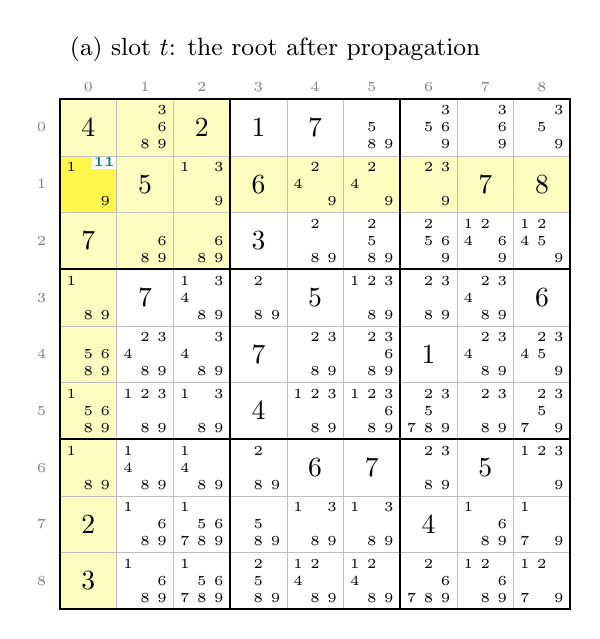
\begin{tikzpicture}[x=1cm,y=1cm]
\node[anchor=south west,font=\small] at (0,6.830) {(a) slot $t$: the root after propagation};
\fill[yellow!25] (0.000,5.760) rectangle (0.720,6.480);
\node[font=\normalsize,text=black] at (0.360,6.120) {4};
\fill[yellow!25] (0.720,5.760) rectangle (1.440,6.480);
\node[font=\tiny,text=black,inner sep=0] at (1.296,6.336) {3};
\node[font=\tiny,text=black,inner sep=0] at (1.296,6.120) {6};
\node[font=\tiny,text=black,inner sep=0] at (1.080,5.904) {8};
\node[font=\tiny,text=black,inner sep=0] at (1.296,5.904) {9};
\fill[yellow!25] (1.440,5.760) rectangle (2.160,6.480);
\node[font=\normalsize,text=black] at (1.800,6.120) {2};
\node[font=\normalsize,text=black] at (2.520,6.120) {1};
\node[font=\normalsize,text=black] at (3.240,6.120) {7};
\node[font=\tiny,text=black,inner sep=0] at (3.960,6.120) {5};
\node[font=\tiny,text=black,inner sep=0] at (3.960,5.904) {8};
\node[font=\tiny,text=black,inner sep=0] at (4.176,5.904) {9};
\node[font=\tiny,text=black,inner sep=0] at (4.896,6.336) {3};
\node[font=\tiny,text=black,inner sep=0] at (4.680,6.120) {5};
\node[font=\tiny,text=black,inner sep=0] at (4.896,6.120) {6};
\node[font=\tiny,text=black,inner sep=0] at (4.896,5.904) {9};
\node[font=\tiny,text=black,inner sep=0] at (5.616,6.336) {3};
\node[font=\tiny,text=black,inner sep=0] at (5.616,6.120) {6};
\node[font=\tiny,text=black,inner sep=0] at (5.616,5.904) {9};
\node[font=\tiny,text=black,inner sep=0] at (6.336,6.336) {3};
\node[font=\tiny,text=black,inner sep=0] at (6.120,6.120) {5};
\node[font=\tiny,text=black,inner sep=0] at (6.336,5.904) {9};
\fill[yellow!70] (0.000,5.040) rectangle (0.720,5.760);
\node[font=\tiny,text=black,inner sep=0] at (0.144,5.616) {1};
\node[font=\tiny,text=black,inner sep=0] at (0.576,5.184) {9};
\node[font=\tiny\bfseries,text=teal,fill=white,anchor=north east,inner sep=0.6pt] at (0.720,5.760) {11};
\fill[yellow!25] (0.720,5.040) rectangle (1.440,5.760);
\node[font=\normalsize,text=black] at (1.080,5.400) {5};
\fill[yellow!25] (1.440,5.040) rectangle (2.160,5.760);
\node[font=\tiny,text=black,inner sep=0] at (1.584,5.616) {1};
\node[font=\tiny,text=black,inner sep=0] at (2.016,5.616) {3};
\node[font=\tiny,text=black,inner sep=0] at (2.016,5.184) {9};
\fill[yellow!25] (2.160,5.040) rectangle (2.880,5.760);
\node[font=\normalsize,text=black] at (2.520,5.400) {6};
\fill[yellow!25] (2.880,5.040) rectangle (3.600,5.760);
\node[font=\tiny,text=black,inner sep=0] at (3.240,5.616) {2};
\node[font=\tiny,text=black,inner sep=0] at (3.024,5.400) {4};
\node[font=\tiny,text=black,inner sep=0] at (3.456,5.184) {9};
\fill[yellow!25] (3.600,5.040) rectangle (4.320,5.760);
\node[font=\tiny,text=black,inner sep=0] at (3.960,5.616) {2};
\node[font=\tiny,text=black,inner sep=0] at (3.744,5.400) {4};
\node[font=\tiny,text=black,inner sep=0] at (4.176,5.184) {9};
\fill[yellow!25] (4.320,5.040) rectangle (5.040,5.760);
\node[font=\tiny,text=black,inner sep=0] at (4.680,5.616) {2};
\node[font=\tiny,text=black,inner sep=0] at (4.896,5.616) {3};
\node[font=\tiny,text=black,inner sep=0] at (4.896,5.184) {9};
\fill[yellow!25] (5.040,5.040) rectangle (5.760,5.760);
\node[font=\normalsize,text=black] at (5.400,5.400) {7};
\fill[yellow!25] (5.760,5.040) rectangle (6.480,5.760);
\node[font=\normalsize,text=black] at (6.120,5.400) {8};
\fill[yellow!25] (0.000,4.320) rectangle (0.720,5.040);
\node[font=\normalsize,text=black] at (0.360,4.680) {7};
\fill[yellow!25] (0.720,4.320) rectangle (1.440,5.040);
\node[font=\tiny,text=black,inner sep=0] at (1.296,4.680) {6};
\node[font=\tiny,text=black,inner sep=0] at (1.080,4.464) {8};
\node[font=\tiny,text=black,inner sep=0] at (1.296,4.464) {9};
\fill[yellow!25] (1.440,4.320) rectangle (2.160,5.040);
\node[font=\tiny,text=black,inner sep=0] at (2.016,4.680) {6};
\node[font=\tiny,text=black,inner sep=0] at (1.800,4.464) {8};
\node[font=\tiny,text=black,inner sep=0] at (2.016,4.464) {9};
\node[font=\normalsize,text=black] at (2.520,4.680) {3};
\node[font=\tiny,text=black,inner sep=0] at (3.240,4.896) {2};
\node[font=\tiny,text=black,inner sep=0] at (3.240,4.464) {8};
\node[font=\tiny,text=black,inner sep=0] at (3.456,4.464) {9};
\node[font=\tiny,text=black,inner sep=0] at (3.960,4.896) {2};
\node[font=\tiny,text=black,inner sep=0] at (3.960,4.680) {5};
\node[font=\tiny,text=black,inner sep=0] at (3.960,4.464) {8};
\node[font=\tiny,text=black,inner sep=0] at (4.176,4.464) {9};
\node[font=\tiny,text=black,inner sep=0] at (4.680,4.896) {2};
\node[font=\tiny,text=black,inner sep=0] at (4.680,4.680) {5};
\node[font=\tiny,text=black,inner sep=0] at (4.896,4.680) {6};
\node[font=\tiny,text=black,inner sep=0] at (4.896,4.464) {9};
\node[font=\tiny,text=black,inner sep=0] at (5.184,4.896) {1};
\node[font=\tiny,text=black,inner sep=0] at (5.400,4.896) {2};
\node[font=\tiny,text=black,inner sep=0] at (5.184,4.680) {4};
\node[font=\tiny,text=black,inner sep=0] at (5.616,4.680) {6};
\node[font=\tiny,text=black,inner sep=0] at (5.616,4.464) {9};
\node[font=\tiny,text=black,inner sep=0] at (5.904,4.896) {1};
\node[font=\tiny,text=black,inner sep=0] at (6.120,4.896) {2};
\node[font=\tiny,text=black,inner sep=0] at (5.904,4.680) {4};
\node[font=\tiny,text=black,inner sep=0] at (6.120,4.680) {5};
\node[font=\tiny,text=black,inner sep=0] at (6.336,4.464) {9};
\fill[yellow!25] (0.000,3.600) rectangle (0.720,4.320);
\node[font=\tiny,text=black,inner sep=0] at (0.144,4.176) {1};
\node[font=\tiny,text=black,inner sep=0] at (0.360,3.744) {8};
\node[font=\tiny,text=black,inner sep=0] at (0.576,3.744) {9};
\node[font=\normalsize,text=black] at (1.080,3.960) {7};
\node[font=\tiny,text=black,inner sep=0] at (1.584,4.176) {1};
\node[font=\tiny,text=black,inner sep=0] at (2.016,4.176) {3};
\node[font=\tiny,text=black,inner sep=0] at (1.584,3.960) {4};
\node[font=\tiny,text=black,inner sep=0] at (1.800,3.744) {8};
\node[font=\tiny,text=black,inner sep=0] at (2.016,3.744) {9};
\node[font=\tiny,text=black,inner sep=0] at (2.520,4.176) {2};
\node[font=\tiny,text=black,inner sep=0] at (2.520,3.744) {8};
\node[font=\tiny,text=black,inner sep=0] at (2.736,3.744) {9};
\node[font=\normalsize,text=black] at (3.240,3.960) {5};
\node[font=\tiny,text=black,inner sep=0] at (3.744,4.176) {1};
\node[font=\tiny,text=black,inner sep=0] at (3.960,4.176) {2};
\node[font=\tiny,text=black,inner sep=0] at (4.176,4.176) {3};
\node[font=\tiny,text=black,inner sep=0] at (3.960,3.744) {8};
\node[font=\tiny,text=black,inner sep=0] at (4.176,3.744) {9};
\node[font=\tiny,text=black,inner sep=0] at (4.680,4.176) {2};
\node[font=\tiny,text=black,inner sep=0] at (4.896,4.176) {3};
\node[font=\tiny,text=black,inner sep=0] at (4.680,3.744) {8};
\node[font=\tiny,text=black,inner sep=0] at (4.896,3.744) {9};
\node[font=\tiny,text=black,inner sep=0] at (5.400,4.176) {2};
\node[font=\tiny,text=black,inner sep=0] at (5.616,4.176) {3};
\node[font=\tiny,text=black,inner sep=0] at (5.184,3.960) {4};
\node[font=\tiny,text=black,inner sep=0] at (5.400,3.744) {8};
\node[font=\tiny,text=black,inner sep=0] at (5.616,3.744) {9};
\node[font=\normalsize,text=black] at (6.120,3.960) {6};
\fill[yellow!25] (0.000,2.880) rectangle (0.720,3.600);
\node[font=\tiny,text=black,inner sep=0] at (0.360,3.240) {5};
\node[font=\tiny,text=black,inner sep=0] at (0.576,3.240) {6};
\node[font=\tiny,text=black,inner sep=0] at (0.360,3.024) {8};
\node[font=\tiny,text=black,inner sep=0] at (0.576,3.024) {9};
\node[font=\tiny,text=black,inner sep=0] at (1.080,3.456) {2};
\node[font=\tiny,text=black,inner sep=0] at (1.296,3.456) {3};
\node[font=\tiny,text=black,inner sep=0] at (0.864,3.240) {4};
\node[font=\tiny,text=black,inner sep=0] at (1.080,3.024) {8};
\node[font=\tiny,text=black,inner sep=0] at (1.296,3.024) {9};
\node[font=\tiny,text=black,inner sep=0] at (2.016,3.456) {3};
\node[font=\tiny,text=black,inner sep=0] at (1.584,3.240) {4};
\node[font=\tiny,text=black,inner sep=0] at (1.800,3.024) {8};
\node[font=\tiny,text=black,inner sep=0] at (2.016,3.024) {9};
\node[font=\normalsize,text=black] at (2.520,3.240) {7};
\node[font=\tiny,text=black,inner sep=0] at (3.240,3.456) {2};
\node[font=\tiny,text=black,inner sep=0] at (3.456,3.456) {3};
\node[font=\tiny,text=black,inner sep=0] at (3.240,3.024) {8};
\node[font=\tiny,text=black,inner sep=0] at (3.456,3.024) {9};
\node[font=\tiny,text=black,inner sep=0] at (3.960,3.456) {2};
\node[font=\tiny,text=black,inner sep=0] at (4.176,3.456) {3};
\node[font=\tiny,text=black,inner sep=0] at (4.176,3.240) {6};
\node[font=\tiny,text=black,inner sep=0] at (3.960,3.024) {8};
\node[font=\tiny,text=black,inner sep=0] at (4.176,3.024) {9};
\node[font=\normalsize,text=black] at (4.680,3.240) {1};
\node[font=\tiny,text=black,inner sep=0] at (5.400,3.456) {2};
\node[font=\tiny,text=black,inner sep=0] at (5.616,3.456) {3};
\node[font=\tiny,text=black,inner sep=0] at (5.184,3.240) {4};
\node[font=\tiny,text=black,inner sep=0] at (5.400,3.024) {8};
\node[font=\tiny,text=black,inner sep=0] at (5.616,3.024) {9};
\node[font=\tiny,text=black,inner sep=0] at (6.120,3.456) {2};
\node[font=\tiny,text=black,inner sep=0] at (6.336,3.456) {3};
\node[font=\tiny,text=black,inner sep=0] at (5.904,3.240) {4};
\node[font=\tiny,text=black,inner sep=0] at (6.120,3.240) {5};
\node[font=\tiny,text=black,inner sep=0] at (6.336,3.024) {9};
\fill[yellow!25] (0.000,2.160) rectangle (0.720,2.880);
\node[font=\tiny,text=black,inner sep=0] at (0.144,2.736) {1};
\node[font=\tiny,text=black,inner sep=0] at (0.360,2.520) {5};
\node[font=\tiny,text=black,inner sep=0] at (0.576,2.520) {6};
\node[font=\tiny,text=black,inner sep=0] at (0.360,2.304) {8};
\node[font=\tiny,text=black,inner sep=0] at (0.576,2.304) {9};
\node[font=\tiny,text=black,inner sep=0] at (0.864,2.736) {1};
\node[font=\tiny,text=black,inner sep=0] at (1.080,2.736) {2};
\node[font=\tiny,text=black,inner sep=0] at (1.296,2.736) {3};
\node[font=\tiny,text=black,inner sep=0] at (1.080,2.304) {8};
\node[font=\tiny,text=black,inner sep=0] at (1.296,2.304) {9};
\node[font=\tiny,text=black,inner sep=0] at (1.584,2.736) {1};
\node[font=\tiny,text=black,inner sep=0] at (2.016,2.736) {3};
\node[font=\tiny,text=black,inner sep=0] at (1.800,2.304) {8};
\node[font=\tiny,text=black,inner sep=0] at (2.016,2.304) {9};
\node[font=\normalsize,text=black] at (2.520,2.520) {4};
\node[font=\tiny,text=black,inner sep=0] at (3.024,2.736) {1};
\node[font=\tiny,text=black,inner sep=0] at (3.240,2.736) {2};
\node[font=\tiny,text=black,inner sep=0] at (3.456,2.736) {3};
\node[font=\tiny,text=black,inner sep=0] at (3.240,2.304) {8};
\node[font=\tiny,text=black,inner sep=0] at (3.456,2.304) {9};
\node[font=\tiny,text=black,inner sep=0] at (3.744,2.736) {1};
\node[font=\tiny,text=black,inner sep=0] at (3.960,2.736) {2};
\node[font=\tiny,text=black,inner sep=0] at (4.176,2.736) {3};
\node[font=\tiny,text=black,inner sep=0] at (4.176,2.520) {6};
\node[font=\tiny,text=black,inner sep=0] at (3.960,2.304) {8};
\node[font=\tiny,text=black,inner sep=0] at (4.176,2.304) {9};
\node[font=\tiny,text=black,inner sep=0] at (4.680,2.736) {2};
\node[font=\tiny,text=black,inner sep=0] at (4.896,2.736) {3};
\node[font=\tiny,text=black,inner sep=0] at (4.680,2.520) {5};
\node[font=\tiny,text=black,inner sep=0] at (4.464,2.304) {7};
\node[font=\tiny,text=black,inner sep=0] at (4.680,2.304) {8};
\node[font=\tiny,text=black,inner sep=0] at (4.896,2.304) {9};
\node[font=\tiny,text=black,inner sep=0] at (5.400,2.736) {2};
\node[font=\tiny,text=black,inner sep=0] at (5.616,2.736) {3};
\node[font=\tiny,text=black,inner sep=0] at (5.400,2.304) {8};
\node[font=\tiny,text=black,inner sep=0] at (5.616,2.304) {9};
\node[font=\tiny,text=black,inner sep=0] at (6.120,2.736) {2};
\node[font=\tiny,text=black,inner sep=0] at (6.336,2.736) {3};
\node[font=\tiny,text=black,inner sep=0] at (6.120,2.520) {5};
\node[font=\tiny,text=black,inner sep=0] at (5.904,2.304) {7};
\node[font=\tiny,text=black,inner sep=0] at (6.336,2.304) {9};
\fill[yellow!25] (0.000,1.440) rectangle (0.720,2.160);
\node[font=\tiny,text=black,inner sep=0] at (0.144,2.016) {1};
\node[font=\tiny,text=black,inner sep=0] at (0.360,1.584) {8};
\node[font=\tiny,text=black,inner sep=0] at (0.576,1.584) {9};
\node[font=\tiny,text=black,inner sep=0] at (0.864,2.016) {1};
\node[font=\tiny,text=black,inner sep=0] at (0.864,1.800) {4};
\node[font=\tiny,text=black,inner sep=0] at (1.080,1.584) {8};
\node[font=\tiny,text=black,inner sep=0] at (1.296,1.584) {9};
\node[font=\tiny,text=black,inner sep=0] at (1.584,2.016) {1};
\node[font=\tiny,text=black,inner sep=0] at (1.584,1.800) {4};
\node[font=\tiny,text=black,inner sep=0] at (1.800,1.584) {8};
\node[font=\tiny,text=black,inner sep=0] at (2.016,1.584) {9};
\node[font=\tiny,text=black,inner sep=0] at (2.520,2.016) {2};
\node[font=\tiny,text=black,inner sep=0] at (2.520,1.584) {8};
\node[font=\tiny,text=black,inner sep=0] at (2.736,1.584) {9};
\node[font=\normalsize,text=black] at (3.240,1.800) {6};
\node[font=\normalsize,text=black] at (3.960,1.800) {7};
\node[font=\tiny,text=black,inner sep=0] at (4.680,2.016) {2};
\node[font=\tiny,text=black,inner sep=0] at (4.896,2.016) {3};
\node[font=\tiny,text=black,inner sep=0] at (4.680,1.584) {8};
\node[font=\tiny,text=black,inner sep=0] at (4.896,1.584) {9};
\node[font=\normalsize,text=black] at (5.400,1.800) {5};
\node[font=\tiny,text=black,inner sep=0] at (5.904,2.016) {1};
\node[font=\tiny,text=black,inner sep=0] at (6.120,2.016) {2};
\node[font=\tiny,text=black,inner sep=0] at (6.336,2.016) {3};
\node[font=\tiny,text=black,inner sep=0] at (6.336,1.584) {9};
\fill[yellow!25] (0.000,0.720) rectangle (0.720,1.440);
\node[font=\normalsize,text=black] at (0.360,1.080) {2};
\node[font=\tiny,text=black,inner sep=0] at (0.864,1.296) {1};
\node[font=\tiny,text=black,inner sep=0] at (1.296,1.080) {6};
\node[font=\tiny,text=black,inner sep=0] at (1.080,0.864) {8};
\node[font=\tiny,text=black,inner sep=0] at (1.296,0.864) {9};
\node[font=\tiny,text=black,inner sep=0] at (1.584,1.296) {1};
\node[font=\tiny,text=black,inner sep=0] at (1.800,1.080) {5};
\node[font=\tiny,text=black,inner sep=0] at (2.016,1.080) {6};
\node[font=\tiny,text=black,inner sep=0] at (1.584,0.864) {7};
\node[font=\tiny,text=black,inner sep=0] at (1.800,0.864) {8};
\node[font=\tiny,text=black,inner sep=0] at (2.016,0.864) {9};
\node[font=\tiny,text=black,inner sep=0] at (2.520,1.080) {5};
\node[font=\tiny,text=black,inner sep=0] at (2.520,0.864) {8};
\node[font=\tiny,text=black,inner sep=0] at (2.736,0.864) {9};
\node[font=\tiny,text=black,inner sep=0] at (3.024,1.296) {1};
\node[font=\tiny,text=black,inner sep=0] at (3.456,1.296) {3};
\node[font=\tiny,text=black,inner sep=0] at (3.240,0.864) {8};
\node[font=\tiny,text=black,inner sep=0] at (3.456,0.864) {9};
\node[font=\tiny,text=black,inner sep=0] at (3.744,1.296) {1};
\node[font=\tiny,text=black,inner sep=0] at (4.176,1.296) {3};
\node[font=\tiny,text=black,inner sep=0] at (3.960,0.864) {8};
\node[font=\tiny,text=black,inner sep=0] at (4.176,0.864) {9};
\node[font=\normalsize,text=black] at (4.680,1.080) {4};
\node[font=\tiny,text=black,inner sep=0] at (5.184,1.296) {1};
\node[font=\tiny,text=black,inner sep=0] at (5.616,1.080) {6};
\node[font=\tiny,text=black,inner sep=0] at (5.400,0.864) {8};
\node[font=\tiny,text=black,inner sep=0] at (5.616,0.864) {9};
\node[font=\tiny,text=black,inner sep=0] at (5.904,1.296) {1};
\node[font=\tiny,text=black,inner sep=0] at (5.904,0.864) {7};
\node[font=\tiny,text=black,inner sep=0] at (6.336,0.864) {9};
\fill[yellow!25] (0.000,0.000) rectangle (0.720,0.720);
\node[font=\normalsize,text=black] at (0.360,0.360) {3};
\node[font=\tiny,text=black,inner sep=0] at (0.864,0.576) {1};
\node[font=\tiny,text=black,inner sep=0] at (1.296,0.360) {6};
\node[font=\tiny,text=black,inner sep=0] at (1.080,0.144) {8};
\node[font=\tiny,text=black,inner sep=0] at (1.296,0.144) {9};
\node[font=\tiny,text=black,inner sep=0] at (1.584,0.576) {1};
\node[font=\tiny,text=black,inner sep=0] at (1.800,0.360) {5};
\node[font=\tiny,text=black,inner sep=0] at (2.016,0.360) {6};
\node[font=\tiny,text=black,inner sep=0] at (1.584,0.144) {7};
\node[font=\tiny,text=black,inner sep=0] at (1.800,0.144) {8};
\node[font=\tiny,text=black,inner sep=0] at (2.016,0.144) {9};
\node[font=\tiny,text=black,inner sep=0] at (2.520,0.576) {2};
\node[font=\tiny,text=black,inner sep=0] at (2.520,0.360) {5};
\node[font=\tiny,text=black,inner sep=0] at (2.520,0.144) {8};
\node[font=\tiny,text=black,inner sep=0] at (2.736,0.144) {9};
\node[font=\tiny,text=black,inner sep=0] at (3.024,0.576) {1};
\node[font=\tiny,text=black,inner sep=0] at (3.240,0.576) {2};
\node[font=\tiny,text=black,inner sep=0] at (3.024,0.360) {4};
\node[font=\tiny,text=black,inner sep=0] at (3.240,0.144) {8};
\node[font=\tiny,text=black,inner sep=0] at (3.456,0.144) {9};
\node[font=\tiny,text=black,inner sep=0] at (3.744,0.576) {1};
\node[font=\tiny,text=black,inner sep=0] at (3.960,0.576) {2};
\node[font=\tiny,text=black,inner sep=0] at (3.744,0.360) {4};
\node[font=\tiny,text=black,inner sep=0] at (3.960,0.144) {8};
\node[font=\tiny,text=black,inner sep=0] at (4.176,0.144) {9};
\node[font=\tiny,text=black,inner sep=0] at (4.680,0.576) {2};
\node[font=\tiny,text=black,inner sep=0] at (4.896,0.360) {6};
\node[font=\tiny,text=black,inner sep=0] at (4.464,0.144) {7};
\node[font=\tiny,text=black,inner sep=0] at (4.680,0.144) {8};
\node[font=\tiny,text=black,inner sep=0] at (4.896,0.144) {9};
\node[font=\tiny,text=black,inner sep=0] at (5.184,0.576) {1};
\node[font=\tiny,text=black,inner sep=0] at (5.400,0.576) {2};
\node[font=\tiny,text=black,inner sep=0] at (5.616,0.360) {6};
\node[font=\tiny,text=black,inner sep=0] at (5.400,0.144) {8};
\node[font=\tiny,text=black,inner sep=0] at (5.616,0.144) {9};
\node[font=\tiny,text=black,inner sep=0] at (5.904,0.576) {1};
\node[font=\tiny,text=black,inner sep=0] at (6.120,0.576) {2};
\node[font=\tiny,text=black,inner sep=0] at (5.904,0.144) {7};
\node[font=\tiny,text=black,inner sep=0] at (6.336,0.144) {9};
\draw[step=0.72,gray!50,very thin] (0,0) grid (6.480,6.480);
\draw[thick] (2.160,0) -- (2.160,6.480);
\draw[thick] (4.320,0) -- (4.320,6.480);
\draw[thick] (0,4.320) -- (6.480,4.320);
\draw[thick] (0,2.160) -- (6.480,2.160);
\draw[thick] (0,0) rectangle (6.480,6.480);
\node[font=\tiny,text=gray] at (0.360,6.630) {0};
\node[font=\tiny,text=gray] at (1.080,6.630) {1};
\node[font=\tiny,text=gray] at (1.800,6.630) {2};
\node[font=\tiny,text=gray] at (2.520,6.630) {3};
\node[font=\tiny,text=gray] at (3.240,6.630) {4};
\node[font=\tiny,text=gray] at (3.960,6.630) {5};
\node[font=\tiny,text=gray] at (4.680,6.630) {6};
\node[font=\tiny,text=gray] at (5.400,6.630) {7};
\node[font=\tiny,text=gray] at (6.120,6.630) {8};
\node[font=\tiny,text=gray,anchor=east] at (-0.05,6.120) {0};
\node[font=\tiny,text=gray,anchor=east] at (-0.05,5.400) {1};
\node[font=\tiny,text=gray,anchor=east] at (-0.05,4.680) {2};
\node[font=\tiny,text=gray,anchor=east] at (-0.05,3.960) {3};
\node[font=\tiny,text=gray,anchor=east] at (-0.05,3.240) {4};
\node[font=\tiny,text=gray,anchor=east] at (-0.05,2.520) {5};
\node[font=\tiny,text=gray,anchor=east] at (-0.05,1.800) {6};
\node[font=\tiny,text=gray,anchor=east] at (-0.05,1.080) {7};
\node[font=\tiny,text=gray,anchor=east] at (-0.05,0.360) {8};
\end{tikzpicture}
\\[0.4cm]
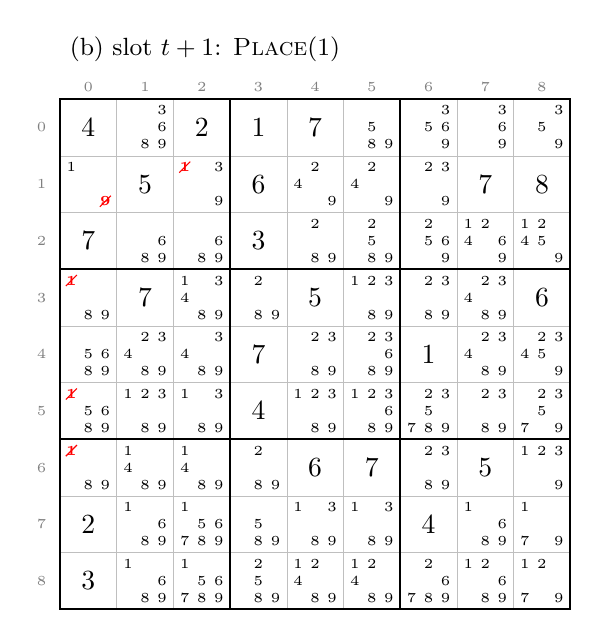
\begin{tikzpicture}[x=1cm,y=1cm]
\node[anchor=south west,font=\small] at (0,6.830) {(b) slot $t+1$: \textsc{Place}(1)};
\node[font=\normalsize,text=black] at (0.360,6.120) {4};
\node[font=\tiny,text=black,inner sep=0] at (1.296,6.336) {3};
\node[font=\tiny,text=black,inner sep=0] at (1.296,6.120) {6};
\node[font=\tiny,text=black,inner sep=0] at (1.080,5.904) {8};
\node[font=\tiny,text=black,inner sep=0] at (1.296,5.904) {9};
\node[font=\normalsize,text=black] at (1.800,6.120) {2};
\node[font=\normalsize,text=black] at (2.520,6.120) {1};
\node[font=\normalsize,text=black] at (3.240,6.120) {7};
\node[font=\tiny,text=black,inner sep=0] at (3.960,6.120) {5};
\node[font=\tiny,text=black,inner sep=0] at (3.960,5.904) {8};
\node[font=\tiny,text=black,inner sep=0] at (4.176,5.904) {9};
\node[font=\tiny,text=black,inner sep=0] at (4.896,6.336) {3};
\node[font=\tiny,text=black,inner sep=0] at (4.680,6.120) {5};
\node[font=\tiny,text=black,inner sep=0] at (4.896,6.120) {6};
\node[font=\tiny,text=black,inner sep=0] at (4.896,5.904) {9};
\node[font=\tiny,text=black,inner sep=0] at (5.616,6.336) {3};
\node[font=\tiny,text=black,inner sep=0] at (5.616,6.120) {6};
\node[font=\tiny,text=black,inner sep=0] at (5.616,5.904) {9};
\node[font=\tiny,text=black,inner sep=0] at (6.336,6.336) {3};
\node[font=\tiny,text=black,inner sep=0] at (6.120,6.120) {5};
\node[font=\tiny,text=black,inner sep=0] at (6.336,5.904) {9};
\node[font=\tiny,text=black,inner sep=0] at (0.144,5.616) {1};
\node[font=\tiny\bfseries,text=red,inner sep=0] at (0.576,5.184) {9};
\draw[red,thin] (0.506,5.114) -- (0.646,5.254);
\node[font=\normalsize,text=black] at (1.080,5.400) {5};
\node[font=\tiny\bfseries,text=red,inner sep=0] at (1.584,5.616) {1};
\draw[red,thin] (1.514,5.546) -- (1.654,5.686);
\node[font=\tiny,text=black,inner sep=0] at (2.016,5.616) {3};
\node[font=\tiny,text=black,inner sep=0] at (2.016,5.184) {9};
\node[font=\normalsize,text=black] at (2.520,5.400) {6};
\node[font=\tiny,text=black,inner sep=0] at (3.240,5.616) {2};
\node[font=\tiny,text=black,inner sep=0] at (3.024,5.400) {4};
\node[font=\tiny,text=black,inner sep=0] at (3.456,5.184) {9};
\node[font=\tiny,text=black,inner sep=0] at (3.960,5.616) {2};
\node[font=\tiny,text=black,inner sep=0] at (3.744,5.400) {4};
\node[font=\tiny,text=black,inner sep=0] at (4.176,5.184) {9};
\node[font=\tiny,text=black,inner sep=0] at (4.680,5.616) {2};
\node[font=\tiny,text=black,inner sep=0] at (4.896,5.616) {3};
\node[font=\tiny,text=black,inner sep=0] at (4.896,5.184) {9};
\node[font=\normalsize,text=black] at (5.400,5.400) {7};
\node[font=\normalsize,text=black] at (6.120,5.400) {8};
\node[font=\normalsize,text=black] at (0.360,4.680) {7};
\node[font=\tiny,text=black,inner sep=0] at (1.296,4.680) {6};
\node[font=\tiny,text=black,inner sep=0] at (1.080,4.464) {8};
\node[font=\tiny,text=black,inner sep=0] at (1.296,4.464) {9};
\node[font=\tiny,text=black,inner sep=0] at (2.016,4.680) {6};
\node[font=\tiny,text=black,inner sep=0] at (1.800,4.464) {8};
\node[font=\tiny,text=black,inner sep=0] at (2.016,4.464) {9};
\node[font=\normalsize,text=black] at (2.520,4.680) {3};
\node[font=\tiny,text=black,inner sep=0] at (3.240,4.896) {2};
\node[font=\tiny,text=black,inner sep=0] at (3.240,4.464) {8};
\node[font=\tiny,text=black,inner sep=0] at (3.456,4.464) {9};
\node[font=\tiny,text=black,inner sep=0] at (3.960,4.896) {2};
\node[font=\tiny,text=black,inner sep=0] at (3.960,4.680) {5};
\node[font=\tiny,text=black,inner sep=0] at (3.960,4.464) {8};
\node[font=\tiny,text=black,inner sep=0] at (4.176,4.464) {9};
\node[font=\tiny,text=black,inner sep=0] at (4.680,4.896) {2};
\node[font=\tiny,text=black,inner sep=0] at (4.680,4.680) {5};
\node[font=\tiny,text=black,inner sep=0] at (4.896,4.680) {6};
\node[font=\tiny,text=black,inner sep=0] at (4.896,4.464) {9};
\node[font=\tiny,text=black,inner sep=0] at (5.184,4.896) {1};
\node[font=\tiny,text=black,inner sep=0] at (5.400,4.896) {2};
\node[font=\tiny,text=black,inner sep=0] at (5.184,4.680) {4};
\node[font=\tiny,text=black,inner sep=0] at (5.616,4.680) {6};
\node[font=\tiny,text=black,inner sep=0] at (5.616,4.464) {9};
\node[font=\tiny,text=black,inner sep=0] at (5.904,4.896) {1};
\node[font=\tiny,text=black,inner sep=0] at (6.120,4.896) {2};
\node[font=\tiny,text=black,inner sep=0] at (5.904,4.680) {4};
\node[font=\tiny,text=black,inner sep=0] at (6.120,4.680) {5};
\node[font=\tiny,text=black,inner sep=0] at (6.336,4.464) {9};
\node[font=\tiny\bfseries,text=red,inner sep=0] at (0.144,4.176) {1};
\draw[red,thin] (0.074,4.106) -- (0.214,4.246);
\node[font=\tiny,text=black,inner sep=0] at (0.360,3.744) {8};
\node[font=\tiny,text=black,inner sep=0] at (0.576,3.744) {9};
\node[font=\normalsize,text=black] at (1.080,3.960) {7};
\node[font=\tiny,text=black,inner sep=0] at (1.584,4.176) {1};
\node[font=\tiny,text=black,inner sep=0] at (2.016,4.176) {3};
\node[font=\tiny,text=black,inner sep=0] at (1.584,3.960) {4};
\node[font=\tiny,text=black,inner sep=0] at (1.800,3.744) {8};
\node[font=\tiny,text=black,inner sep=0] at (2.016,3.744) {9};
\node[font=\tiny,text=black,inner sep=0] at (2.520,4.176) {2};
\node[font=\tiny,text=black,inner sep=0] at (2.520,3.744) {8};
\node[font=\tiny,text=black,inner sep=0] at (2.736,3.744) {9};
\node[font=\normalsize,text=black] at (3.240,3.960) {5};
\node[font=\tiny,text=black,inner sep=0] at (3.744,4.176) {1};
\node[font=\tiny,text=black,inner sep=0] at (3.960,4.176) {2};
\node[font=\tiny,text=black,inner sep=0] at (4.176,4.176) {3};
\node[font=\tiny,text=black,inner sep=0] at (3.960,3.744) {8};
\node[font=\tiny,text=black,inner sep=0] at (4.176,3.744) {9};
\node[font=\tiny,text=black,inner sep=0] at (4.680,4.176) {2};
\node[font=\tiny,text=black,inner sep=0] at (4.896,4.176) {3};
\node[font=\tiny,text=black,inner sep=0] at (4.680,3.744) {8};
\node[font=\tiny,text=black,inner sep=0] at (4.896,3.744) {9};
\node[font=\tiny,text=black,inner sep=0] at (5.400,4.176) {2};
\node[font=\tiny,text=black,inner sep=0] at (5.616,4.176) {3};
\node[font=\tiny,text=black,inner sep=0] at (5.184,3.960) {4};
\node[font=\tiny,text=black,inner sep=0] at (5.400,3.744) {8};
\node[font=\tiny,text=black,inner sep=0] at (5.616,3.744) {9};
\node[font=\normalsize,text=black] at (6.120,3.960) {6};
\node[font=\tiny,text=black,inner sep=0] at (0.360,3.240) {5};
\node[font=\tiny,text=black,inner sep=0] at (0.576,3.240) {6};
\node[font=\tiny,text=black,inner sep=0] at (0.360,3.024) {8};
\node[font=\tiny,text=black,inner sep=0] at (0.576,3.024) {9};
\node[font=\tiny,text=black,inner sep=0] at (1.080,3.456) {2};
\node[font=\tiny,text=black,inner sep=0] at (1.296,3.456) {3};
\node[font=\tiny,text=black,inner sep=0] at (0.864,3.240) {4};
\node[font=\tiny,text=black,inner sep=0] at (1.080,3.024) {8};
\node[font=\tiny,text=black,inner sep=0] at (1.296,3.024) {9};
\node[font=\tiny,text=black,inner sep=0] at (2.016,3.456) {3};
\node[font=\tiny,text=black,inner sep=0] at (1.584,3.240) {4};
\node[font=\tiny,text=black,inner sep=0] at (1.800,3.024) {8};
\node[font=\tiny,text=black,inner sep=0] at (2.016,3.024) {9};
\node[font=\normalsize,text=black] at (2.520,3.240) {7};
\node[font=\tiny,text=black,inner sep=0] at (3.240,3.456) {2};
\node[font=\tiny,text=black,inner sep=0] at (3.456,3.456) {3};
\node[font=\tiny,text=black,inner sep=0] at (3.240,3.024) {8};
\node[font=\tiny,text=black,inner sep=0] at (3.456,3.024) {9};
\node[font=\tiny,text=black,inner sep=0] at (3.960,3.456) {2};
\node[font=\tiny,text=black,inner sep=0] at (4.176,3.456) {3};
\node[font=\tiny,text=black,inner sep=0] at (4.176,3.240) {6};
\node[font=\tiny,text=black,inner sep=0] at (3.960,3.024) {8};
\node[font=\tiny,text=black,inner sep=0] at (4.176,3.024) {9};
\node[font=\normalsize,text=black] at (4.680,3.240) {1};
\node[font=\tiny,text=black,inner sep=0] at (5.400,3.456) {2};
\node[font=\tiny,text=black,inner sep=0] at (5.616,3.456) {3};
\node[font=\tiny,text=black,inner sep=0] at (5.184,3.240) {4};
\node[font=\tiny,text=black,inner sep=0] at (5.400,3.024) {8};
\node[font=\tiny,text=black,inner sep=0] at (5.616,3.024) {9};
\node[font=\tiny,text=black,inner sep=0] at (6.120,3.456) {2};
\node[font=\tiny,text=black,inner sep=0] at (6.336,3.456) {3};
\node[font=\tiny,text=black,inner sep=0] at (5.904,3.240) {4};
\node[font=\tiny,text=black,inner sep=0] at (6.120,3.240) {5};
\node[font=\tiny,text=black,inner sep=0] at (6.336,3.024) {9};
\node[font=\tiny\bfseries,text=red,inner sep=0] at (0.144,2.736) {1};
\draw[red,thin] (0.074,2.666) -- (0.214,2.806);
\node[font=\tiny,text=black,inner sep=0] at (0.360,2.520) {5};
\node[font=\tiny,text=black,inner sep=0] at (0.576,2.520) {6};
\node[font=\tiny,text=black,inner sep=0] at (0.360,2.304) {8};
\node[font=\tiny,text=black,inner sep=0] at (0.576,2.304) {9};
\node[font=\tiny,text=black,inner sep=0] at (0.864,2.736) {1};
\node[font=\tiny,text=black,inner sep=0] at (1.080,2.736) {2};
\node[font=\tiny,text=black,inner sep=0] at (1.296,2.736) {3};
\node[font=\tiny,text=black,inner sep=0] at (1.080,2.304) {8};
\node[font=\tiny,text=black,inner sep=0] at (1.296,2.304) {9};
\node[font=\tiny,text=black,inner sep=0] at (1.584,2.736) {1};
\node[font=\tiny,text=black,inner sep=0] at (2.016,2.736) {3};
\node[font=\tiny,text=black,inner sep=0] at (1.800,2.304) {8};
\node[font=\tiny,text=black,inner sep=0] at (2.016,2.304) {9};
\node[font=\normalsize,text=black] at (2.520,2.520) {4};
\node[font=\tiny,text=black,inner sep=0] at (3.024,2.736) {1};
\node[font=\tiny,text=black,inner sep=0] at (3.240,2.736) {2};
\node[font=\tiny,text=black,inner sep=0] at (3.456,2.736) {3};
\node[font=\tiny,text=black,inner sep=0] at (3.240,2.304) {8};
\node[font=\tiny,text=black,inner sep=0] at (3.456,2.304) {9};
\node[font=\tiny,text=black,inner sep=0] at (3.744,2.736) {1};
\node[font=\tiny,text=black,inner sep=0] at (3.960,2.736) {2};
\node[font=\tiny,text=black,inner sep=0] at (4.176,2.736) {3};
\node[font=\tiny,text=black,inner sep=0] at (4.176,2.520) {6};
\node[font=\tiny,text=black,inner sep=0] at (3.960,2.304) {8};
\node[font=\tiny,text=black,inner sep=0] at (4.176,2.304) {9};
\node[font=\tiny,text=black,inner sep=0] at (4.680,2.736) {2};
\node[font=\tiny,text=black,inner sep=0] at (4.896,2.736) {3};
\node[font=\tiny,text=black,inner sep=0] at (4.680,2.520) {5};
\node[font=\tiny,text=black,inner sep=0] at (4.464,2.304) {7};
\node[font=\tiny,text=black,inner sep=0] at (4.680,2.304) {8};
\node[font=\tiny,text=black,inner sep=0] at (4.896,2.304) {9};
\node[font=\tiny,text=black,inner sep=0] at (5.400,2.736) {2};
\node[font=\tiny,text=black,inner sep=0] at (5.616,2.736) {3};
\node[font=\tiny,text=black,inner sep=0] at (5.400,2.304) {8};
\node[font=\tiny,text=black,inner sep=0] at (5.616,2.304) {9};
\node[font=\tiny,text=black,inner sep=0] at (6.120,2.736) {2};
\node[font=\tiny,text=black,inner sep=0] at (6.336,2.736) {3};
\node[font=\tiny,text=black,inner sep=0] at (6.120,2.520) {5};
\node[font=\tiny,text=black,inner sep=0] at (5.904,2.304) {7};
\node[font=\tiny,text=black,inner sep=0] at (6.336,2.304) {9};
\node[font=\tiny\bfseries,text=red,inner sep=0] at (0.144,2.016) {1};
\draw[red,thin] (0.074,1.946) -- (0.214,2.086);
\node[font=\tiny,text=black,inner sep=0] at (0.360,1.584) {8};
\node[font=\tiny,text=black,inner sep=0] at (0.576,1.584) {9};
\node[font=\tiny,text=black,inner sep=0] at (0.864,2.016) {1};
\node[font=\tiny,text=black,inner sep=0] at (0.864,1.800) {4};
\node[font=\tiny,text=black,inner sep=0] at (1.080,1.584) {8};
\node[font=\tiny,text=black,inner sep=0] at (1.296,1.584) {9};
\node[font=\tiny,text=black,inner sep=0] at (1.584,2.016) {1};
\node[font=\tiny,text=black,inner sep=0] at (1.584,1.800) {4};
\node[font=\tiny,text=black,inner sep=0] at (1.800,1.584) {8};
\node[font=\tiny,text=black,inner sep=0] at (2.016,1.584) {9};
\node[font=\tiny,text=black,inner sep=0] at (2.520,2.016) {2};
\node[font=\tiny,text=black,inner sep=0] at (2.520,1.584) {8};
\node[font=\tiny,text=black,inner sep=0] at (2.736,1.584) {9};
\node[font=\normalsize,text=black] at (3.240,1.800) {6};
\node[font=\normalsize,text=black] at (3.960,1.800) {7};
\node[font=\tiny,text=black,inner sep=0] at (4.680,2.016) {2};
\node[font=\tiny,text=black,inner sep=0] at (4.896,2.016) {3};
\node[font=\tiny,text=black,inner sep=0] at (4.680,1.584) {8};
\node[font=\tiny,text=black,inner sep=0] at (4.896,1.584) {9};
\node[font=\normalsize,text=black] at (5.400,1.800) {5};
\node[font=\tiny,text=black,inner sep=0] at (5.904,2.016) {1};
\node[font=\tiny,text=black,inner sep=0] at (6.120,2.016) {2};
\node[font=\tiny,text=black,inner sep=0] at (6.336,2.016) {3};
\node[font=\tiny,text=black,inner sep=0] at (6.336,1.584) {9};
\node[font=\normalsize,text=black] at (0.360,1.080) {2};
\node[font=\tiny,text=black,inner sep=0] at (0.864,1.296) {1};
\node[font=\tiny,text=black,inner sep=0] at (1.296,1.080) {6};
\node[font=\tiny,text=black,inner sep=0] at (1.080,0.864) {8};
\node[font=\tiny,text=black,inner sep=0] at (1.296,0.864) {9};
\node[font=\tiny,text=black,inner sep=0] at (1.584,1.296) {1};
\node[font=\tiny,text=black,inner sep=0] at (1.800,1.080) {5};
\node[font=\tiny,text=black,inner sep=0] at (2.016,1.080) {6};
\node[font=\tiny,text=black,inner sep=0] at (1.584,0.864) {7};
\node[font=\tiny,text=black,inner sep=0] at (1.800,0.864) {8};
\node[font=\tiny,text=black,inner sep=0] at (2.016,0.864) {9};
\node[font=\tiny,text=black,inner sep=0] at (2.520,1.080) {5};
\node[font=\tiny,text=black,inner sep=0] at (2.520,0.864) {8};
\node[font=\tiny,text=black,inner sep=0] at (2.736,0.864) {9};
\node[font=\tiny,text=black,inner sep=0] at (3.024,1.296) {1};
\node[font=\tiny,text=black,inner sep=0] at (3.456,1.296) {3};
\node[font=\tiny,text=black,inner sep=0] at (3.240,0.864) {8};
\node[font=\tiny,text=black,inner sep=0] at (3.456,0.864) {9};
\node[font=\tiny,text=black,inner sep=0] at (3.744,1.296) {1};
\node[font=\tiny,text=black,inner sep=0] at (4.176,1.296) {3};
\node[font=\tiny,text=black,inner sep=0] at (3.960,0.864) {8};
\node[font=\tiny,text=black,inner sep=0] at (4.176,0.864) {9};
\node[font=\normalsize,text=black] at (4.680,1.080) {4};
\node[font=\tiny,text=black,inner sep=0] at (5.184,1.296) {1};
\node[font=\tiny,text=black,inner sep=0] at (5.616,1.080) {6};
\node[font=\tiny,text=black,inner sep=0] at (5.400,0.864) {8};
\node[font=\tiny,text=black,inner sep=0] at (5.616,0.864) {9};
\node[font=\tiny,text=black,inner sep=0] at (5.904,1.296) {1};
\node[font=\tiny,text=black,inner sep=0] at (5.904,0.864) {7};
\node[font=\tiny,text=black,inner sep=0] at (6.336,0.864) {9};
\node[font=\normalsize,text=black] at (0.360,0.360) {3};
\node[font=\tiny,text=black,inner sep=0] at (0.864,0.576) {1};
\node[font=\tiny,text=black,inner sep=0] at (1.296,0.360) {6};
\node[font=\tiny,text=black,inner sep=0] at (1.080,0.144) {8};
\node[font=\tiny,text=black,inner sep=0] at (1.296,0.144) {9};
\node[font=\tiny,text=black,inner sep=0] at (1.584,0.576) {1};
\node[font=\tiny,text=black,inner sep=0] at (1.800,0.360) {5};
\node[font=\tiny,text=black,inner sep=0] at (2.016,0.360) {6};
\node[font=\tiny,text=black,inner sep=0] at (1.584,0.144) {7};
\node[font=\tiny,text=black,inner sep=0] at (1.800,0.144) {8};
\node[font=\tiny,text=black,inner sep=0] at (2.016,0.144) {9};
\node[font=\tiny,text=black,inner sep=0] at (2.520,0.576) {2};
\node[font=\tiny,text=black,inner sep=0] at (2.520,0.360) {5};
\node[font=\tiny,text=black,inner sep=0] at (2.520,0.144) {8};
\node[font=\tiny,text=black,inner sep=0] at (2.736,0.144) {9};
\node[font=\tiny,text=black,inner sep=0] at (3.024,0.576) {1};
\node[font=\tiny,text=black,inner sep=0] at (3.240,0.576) {2};
\node[font=\tiny,text=black,inner sep=0] at (3.024,0.360) {4};
\node[font=\tiny,text=black,inner sep=0] at (3.240,0.144) {8};
\node[font=\tiny,text=black,inner sep=0] at (3.456,0.144) {9};
\node[font=\tiny,text=black,inner sep=0] at (3.744,0.576) {1};
\node[font=\tiny,text=black,inner sep=0] at (3.960,0.576) {2};
\node[font=\tiny,text=black,inner sep=0] at (3.744,0.360) {4};
\node[font=\tiny,text=black,inner sep=0] at (3.960,0.144) {8};
\node[font=\tiny,text=black,inner sep=0] at (4.176,0.144) {9};
\node[font=\tiny,text=black,inner sep=0] at (4.680,0.576) {2};
\node[font=\tiny,text=black,inner sep=0] at (4.896,0.360) {6};
\node[font=\tiny,text=black,inner sep=0] at (4.464,0.144) {7};
\node[font=\tiny,text=black,inner sep=0] at (4.680,0.144) {8};
\node[font=\tiny,text=black,inner sep=0] at (4.896,0.144) {9};
\node[font=\tiny,text=black,inner sep=0] at (5.184,0.576) {1};
\node[font=\tiny,text=black,inner sep=0] at (5.400,0.576) {2};
\node[font=\tiny,text=black,inner sep=0] at (5.616,0.360) {6};
\node[font=\tiny,text=black,inner sep=0] at (5.400,0.144) {8};
\node[font=\tiny,text=black,inner sep=0] at (5.616,0.144) {9};
\node[font=\tiny,text=black,inner sep=0] at (5.904,0.576) {1};
\node[font=\tiny,text=black,inner sep=0] at (6.120,0.576) {2};
\node[font=\tiny,text=black,inner sep=0] at (5.904,0.144) {7};
\node[font=\tiny,text=black,inner sep=0] at (6.336,0.144) {9};
\draw[step=0.72,gray!50,very thin] (0,0) grid (6.480,6.480);
\draw[thick] (2.160,0) -- (2.160,6.480);
\draw[thick] (4.320,0) -- (4.320,6.480);
\draw[thick] (0,4.320) -- (6.480,4.320);
\draw[thick] (0,2.160) -- (6.480,2.160);
\draw[thick] (0,0) rectangle (6.480,6.480);
\node[font=\tiny,text=gray] at (0.360,6.630) {0};
\node[font=\tiny,text=gray] at (1.080,6.630) {1};
\node[font=\tiny,text=gray] at (1.800,6.630) {2};
\node[font=\tiny,text=gray] at (2.520,6.630) {3};
\node[font=\tiny,text=gray] at (3.240,6.630) {4};
\node[font=\tiny,text=gray] at (3.960,6.630) {5};
\node[font=\tiny,text=gray] at (4.680,6.630) {6};
\node[font=\tiny,text=gray] at (5.400,6.630) {7};
\node[font=\tiny,text=gray] at (6.120,6.630) {8};
\node[font=\tiny,text=gray,anchor=east] at (-0.05,6.120) {0};
\node[font=\tiny,text=gray,anchor=east] at (-0.05,5.400) {1};
\node[font=\tiny,text=gray,anchor=east] at (-0.05,4.680) {2};
\node[font=\tiny,text=gray,anchor=east] at (-0.05,3.960) {3};
\node[font=\tiny,text=gray,anchor=east] at (-0.05,3.240) {4};
\node[font=\tiny,text=gray,anchor=east] at (-0.05,2.520) {5};
\node[font=\tiny,text=gray,anchor=east] at (-0.05,1.800) {6};
\node[font=\tiny,text=gray,anchor=east] at (-0.05,1.080) {7};
\node[font=\tiny,text=gray,anchor=east] at (-0.05,0.360) {8};
\end{tikzpicture}
\hspace{0.5cm}
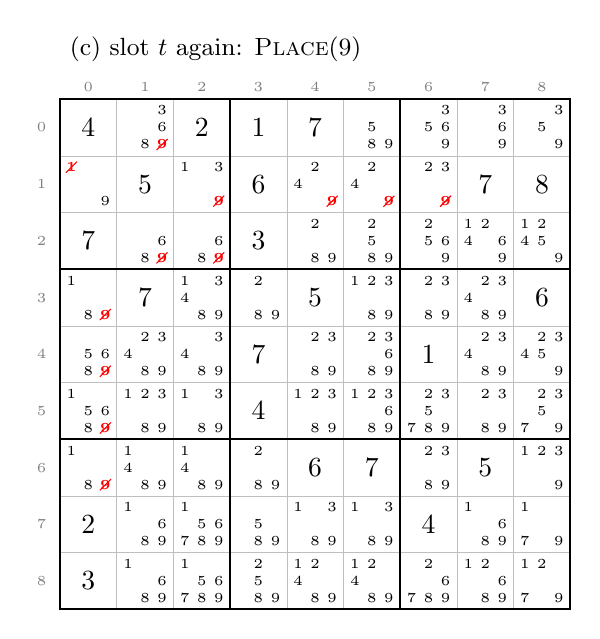
\begin{tikzpicture}[x=1cm,y=1cm]
\node[anchor=south west,font=\small] at (0,6.830) {(c) slot $t$ again: \textsc{Place}(9)};
\node[font=\normalsize,text=black] at (0.360,6.120) {4};
\node[font=\tiny,text=black,inner sep=0] at (1.296,6.336) {3};
\node[font=\tiny,text=black,inner sep=0] at (1.296,6.120) {6};
\node[font=\tiny,text=black,inner sep=0] at (1.080,5.904) {8};
\node[font=\tiny\bfseries,text=red,inner sep=0] at (1.296,5.904) {9};
\draw[red,thin] (1.226,5.834) -- (1.366,5.974);
\node[font=\normalsize,text=black] at (1.800,6.120) {2};
\node[font=\normalsize,text=black] at (2.520,6.120) {1};
\node[font=\normalsize,text=black] at (3.240,6.120) {7};
\node[font=\tiny,text=black,inner sep=0] at (3.960,6.120) {5};
\node[font=\tiny,text=black,inner sep=0] at (3.960,5.904) {8};
\node[font=\tiny,text=black,inner sep=0] at (4.176,5.904) {9};
\node[font=\tiny,text=black,inner sep=0] at (4.896,6.336) {3};
\node[font=\tiny,text=black,inner sep=0] at (4.680,6.120) {5};
\node[font=\tiny,text=black,inner sep=0] at (4.896,6.120) {6};
\node[font=\tiny,text=black,inner sep=0] at (4.896,5.904) {9};
\node[font=\tiny,text=black,inner sep=0] at (5.616,6.336) {3};
\node[font=\tiny,text=black,inner sep=0] at (5.616,6.120) {6};
\node[font=\tiny,text=black,inner sep=0] at (5.616,5.904) {9};
\node[font=\tiny,text=black,inner sep=0] at (6.336,6.336) {3};
\node[font=\tiny,text=black,inner sep=0] at (6.120,6.120) {5};
\node[font=\tiny,text=black,inner sep=0] at (6.336,5.904) {9};
\node[font=\tiny\bfseries,text=red,inner sep=0] at (0.144,5.616) {1};
\draw[red,thin] (0.074,5.546) -- (0.214,5.686);
\node[font=\tiny,text=black,inner sep=0] at (0.576,5.184) {9};
\node[font=\normalsize,text=black] at (1.080,5.400) {5};
\node[font=\tiny,text=black,inner sep=0] at (1.584,5.616) {1};
\node[font=\tiny,text=black,inner sep=0] at (2.016,5.616) {3};
\node[font=\tiny\bfseries,text=red,inner sep=0] at (2.016,5.184) {9};
\draw[red,thin] (1.946,5.114) -- (2.086,5.254);
\node[font=\normalsize,text=black] at (2.520,5.400) {6};
\node[font=\tiny,text=black,inner sep=0] at (3.240,5.616) {2};
\node[font=\tiny,text=black,inner sep=0] at (3.024,5.400) {4};
\node[font=\tiny\bfseries,text=red,inner sep=0] at (3.456,5.184) {9};
\draw[red,thin] (3.386,5.114) -- (3.526,5.254);
\node[font=\tiny,text=black,inner sep=0] at (3.960,5.616) {2};
\node[font=\tiny,text=black,inner sep=0] at (3.744,5.400) {4};
\node[font=\tiny\bfseries,text=red,inner sep=0] at (4.176,5.184) {9};
\draw[red,thin] (4.106,5.114) -- (4.246,5.254);
\node[font=\tiny,text=black,inner sep=0] at (4.680,5.616) {2};
\node[font=\tiny,text=black,inner sep=0] at (4.896,5.616) {3};
\node[font=\tiny\bfseries,text=red,inner sep=0] at (4.896,5.184) {9};
\draw[red,thin] (4.826,5.114) -- (4.966,5.254);
\node[font=\normalsize,text=black] at (5.400,5.400) {7};
\node[font=\normalsize,text=black] at (6.120,5.400) {8};
\node[font=\normalsize,text=black] at (0.360,4.680) {7};
\node[font=\tiny,text=black,inner sep=0] at (1.296,4.680) {6};
\node[font=\tiny,text=black,inner sep=0] at (1.080,4.464) {8};
\node[font=\tiny\bfseries,text=red,inner sep=0] at (1.296,4.464) {9};
\draw[red,thin] (1.226,4.394) -- (1.366,4.534);
\node[font=\tiny,text=black,inner sep=0] at (2.016,4.680) {6};
\node[font=\tiny,text=black,inner sep=0] at (1.800,4.464) {8};
\node[font=\tiny\bfseries,text=red,inner sep=0] at (2.016,4.464) {9};
\draw[red,thin] (1.946,4.394) -- (2.086,4.534);
\node[font=\normalsize,text=black] at (2.520,4.680) {3};
\node[font=\tiny,text=black,inner sep=0] at (3.240,4.896) {2};
\node[font=\tiny,text=black,inner sep=0] at (3.240,4.464) {8};
\node[font=\tiny,text=black,inner sep=0] at (3.456,4.464) {9};
\node[font=\tiny,text=black,inner sep=0] at (3.960,4.896) {2};
\node[font=\tiny,text=black,inner sep=0] at (3.960,4.680) {5};
\node[font=\tiny,text=black,inner sep=0] at (3.960,4.464) {8};
\node[font=\tiny,text=black,inner sep=0] at (4.176,4.464) {9};
\node[font=\tiny,text=black,inner sep=0] at (4.680,4.896) {2};
\node[font=\tiny,text=black,inner sep=0] at (4.680,4.680) {5};
\node[font=\tiny,text=black,inner sep=0] at (4.896,4.680) {6};
\node[font=\tiny,text=black,inner sep=0] at (4.896,4.464) {9};
\node[font=\tiny,text=black,inner sep=0] at (5.184,4.896) {1};
\node[font=\tiny,text=black,inner sep=0] at (5.400,4.896) {2};
\node[font=\tiny,text=black,inner sep=0] at (5.184,4.680) {4};
\node[font=\tiny,text=black,inner sep=0] at (5.616,4.680) {6};
\node[font=\tiny,text=black,inner sep=0] at (5.616,4.464) {9};
\node[font=\tiny,text=black,inner sep=0] at (5.904,4.896) {1};
\node[font=\tiny,text=black,inner sep=0] at (6.120,4.896) {2};
\node[font=\tiny,text=black,inner sep=0] at (5.904,4.680) {4};
\node[font=\tiny,text=black,inner sep=0] at (6.120,4.680) {5};
\node[font=\tiny,text=black,inner sep=0] at (6.336,4.464) {9};
\node[font=\tiny,text=black,inner sep=0] at (0.144,4.176) {1};
\node[font=\tiny,text=black,inner sep=0] at (0.360,3.744) {8};
\node[font=\tiny\bfseries,text=red,inner sep=0] at (0.576,3.744) {9};
\draw[red,thin] (0.506,3.674) -- (0.646,3.814);
\node[font=\normalsize,text=black] at (1.080,3.960) {7};
\node[font=\tiny,text=black,inner sep=0] at (1.584,4.176) {1};
\node[font=\tiny,text=black,inner sep=0] at (2.016,4.176) {3};
\node[font=\tiny,text=black,inner sep=0] at (1.584,3.960) {4};
\node[font=\tiny,text=black,inner sep=0] at (1.800,3.744) {8};
\node[font=\tiny,text=black,inner sep=0] at (2.016,3.744) {9};
\node[font=\tiny,text=black,inner sep=0] at (2.520,4.176) {2};
\node[font=\tiny,text=black,inner sep=0] at (2.520,3.744) {8};
\node[font=\tiny,text=black,inner sep=0] at (2.736,3.744) {9};
\node[font=\normalsize,text=black] at (3.240,3.960) {5};
\node[font=\tiny,text=black,inner sep=0] at (3.744,4.176) {1};
\node[font=\tiny,text=black,inner sep=0] at (3.960,4.176) {2};
\node[font=\tiny,text=black,inner sep=0] at (4.176,4.176) {3};
\node[font=\tiny,text=black,inner sep=0] at (3.960,3.744) {8};
\node[font=\tiny,text=black,inner sep=0] at (4.176,3.744) {9};
\node[font=\tiny,text=black,inner sep=0] at (4.680,4.176) {2};
\node[font=\tiny,text=black,inner sep=0] at (4.896,4.176) {3};
\node[font=\tiny,text=black,inner sep=0] at (4.680,3.744) {8};
\node[font=\tiny,text=black,inner sep=0] at (4.896,3.744) {9};
\node[font=\tiny,text=black,inner sep=0] at (5.400,4.176) {2};
\node[font=\tiny,text=black,inner sep=0] at (5.616,4.176) {3};
\node[font=\tiny,text=black,inner sep=0] at (5.184,3.960) {4};
\node[font=\tiny,text=black,inner sep=0] at (5.400,3.744) {8};
\node[font=\tiny,text=black,inner sep=0] at (5.616,3.744) {9};
\node[font=\normalsize,text=black] at (6.120,3.960) {6};
\node[font=\tiny,text=black,inner sep=0] at (0.360,3.240) {5};
\node[font=\tiny,text=black,inner sep=0] at (0.576,3.240) {6};
\node[font=\tiny,text=black,inner sep=0] at (0.360,3.024) {8};
\node[font=\tiny\bfseries,text=red,inner sep=0] at (0.576,3.024) {9};
\draw[red,thin] (0.506,2.954) -- (0.646,3.094);
\node[font=\tiny,text=black,inner sep=0] at (1.080,3.456) {2};
\node[font=\tiny,text=black,inner sep=0] at (1.296,3.456) {3};
\node[font=\tiny,text=black,inner sep=0] at (0.864,3.240) {4};
\node[font=\tiny,text=black,inner sep=0] at (1.080,3.024) {8};
\node[font=\tiny,text=black,inner sep=0] at (1.296,3.024) {9};
\node[font=\tiny,text=black,inner sep=0] at (2.016,3.456) {3};
\node[font=\tiny,text=black,inner sep=0] at (1.584,3.240) {4};
\node[font=\tiny,text=black,inner sep=0] at (1.800,3.024) {8};
\node[font=\tiny,text=black,inner sep=0] at (2.016,3.024) {9};
\node[font=\normalsize,text=black] at (2.520,3.240) {7};
\node[font=\tiny,text=black,inner sep=0] at (3.240,3.456) {2};
\node[font=\tiny,text=black,inner sep=0] at (3.456,3.456) {3};
\node[font=\tiny,text=black,inner sep=0] at (3.240,3.024) {8};
\node[font=\tiny,text=black,inner sep=0] at (3.456,3.024) {9};
\node[font=\tiny,text=black,inner sep=0] at (3.960,3.456) {2};
\node[font=\tiny,text=black,inner sep=0] at (4.176,3.456) {3};
\node[font=\tiny,text=black,inner sep=0] at (4.176,3.240) {6};
\node[font=\tiny,text=black,inner sep=0] at (3.960,3.024) {8};
\node[font=\tiny,text=black,inner sep=0] at (4.176,3.024) {9};
\node[font=\normalsize,text=black] at (4.680,3.240) {1};
\node[font=\tiny,text=black,inner sep=0] at (5.400,3.456) {2};
\node[font=\tiny,text=black,inner sep=0] at (5.616,3.456) {3};
\node[font=\tiny,text=black,inner sep=0] at (5.184,3.240) {4};
\node[font=\tiny,text=black,inner sep=0] at (5.400,3.024) {8};
\node[font=\tiny,text=black,inner sep=0] at (5.616,3.024) {9};
\node[font=\tiny,text=black,inner sep=0] at (6.120,3.456) {2};
\node[font=\tiny,text=black,inner sep=0] at (6.336,3.456) {3};
\node[font=\tiny,text=black,inner sep=0] at (5.904,3.240) {4};
\node[font=\tiny,text=black,inner sep=0] at (6.120,3.240) {5};
\node[font=\tiny,text=black,inner sep=0] at (6.336,3.024) {9};
\node[font=\tiny,text=black,inner sep=0] at (0.144,2.736) {1};
\node[font=\tiny,text=black,inner sep=0] at (0.360,2.520) {5};
\node[font=\tiny,text=black,inner sep=0] at (0.576,2.520) {6};
\node[font=\tiny,text=black,inner sep=0] at (0.360,2.304) {8};
\node[font=\tiny\bfseries,text=red,inner sep=0] at (0.576,2.304) {9};
\draw[red,thin] (0.506,2.234) -- (0.646,2.374);
\node[font=\tiny,text=black,inner sep=0] at (0.864,2.736) {1};
\node[font=\tiny,text=black,inner sep=0] at (1.080,2.736) {2};
\node[font=\tiny,text=black,inner sep=0] at (1.296,2.736) {3};
\node[font=\tiny,text=black,inner sep=0] at (1.080,2.304) {8};
\node[font=\tiny,text=black,inner sep=0] at (1.296,2.304) {9};
\node[font=\tiny,text=black,inner sep=0] at (1.584,2.736) {1};
\node[font=\tiny,text=black,inner sep=0] at (2.016,2.736) {3};
\node[font=\tiny,text=black,inner sep=0] at (1.800,2.304) {8};
\node[font=\tiny,text=black,inner sep=0] at (2.016,2.304) {9};
\node[font=\normalsize,text=black] at (2.520,2.520) {4};
\node[font=\tiny,text=black,inner sep=0] at (3.024,2.736) {1};
\node[font=\tiny,text=black,inner sep=0] at (3.240,2.736) {2};
\node[font=\tiny,text=black,inner sep=0] at (3.456,2.736) {3};
\node[font=\tiny,text=black,inner sep=0] at (3.240,2.304) {8};
\node[font=\tiny,text=black,inner sep=0] at (3.456,2.304) {9};
\node[font=\tiny,text=black,inner sep=0] at (3.744,2.736) {1};
\node[font=\tiny,text=black,inner sep=0] at (3.960,2.736) {2};
\node[font=\tiny,text=black,inner sep=0] at (4.176,2.736) {3};
\node[font=\tiny,text=black,inner sep=0] at (4.176,2.520) {6};
\node[font=\tiny,text=black,inner sep=0] at (3.960,2.304) {8};
\node[font=\tiny,text=black,inner sep=0] at (4.176,2.304) {9};
\node[font=\tiny,text=black,inner sep=0] at (4.680,2.736) {2};
\node[font=\tiny,text=black,inner sep=0] at (4.896,2.736) {3};
\node[font=\tiny,text=black,inner sep=0] at (4.680,2.520) {5};
\node[font=\tiny,text=black,inner sep=0] at (4.464,2.304) {7};
\node[font=\tiny,text=black,inner sep=0] at (4.680,2.304) {8};
\node[font=\tiny,text=black,inner sep=0] at (4.896,2.304) {9};
\node[font=\tiny,text=black,inner sep=0] at (5.400,2.736) {2};
\node[font=\tiny,text=black,inner sep=0] at (5.616,2.736) {3};
\node[font=\tiny,text=black,inner sep=0] at (5.400,2.304) {8};
\node[font=\tiny,text=black,inner sep=0] at (5.616,2.304) {9};
\node[font=\tiny,text=black,inner sep=0] at (6.120,2.736) {2};
\node[font=\tiny,text=black,inner sep=0] at (6.336,2.736) {3};
\node[font=\tiny,text=black,inner sep=0] at (6.120,2.520) {5};
\node[font=\tiny,text=black,inner sep=0] at (5.904,2.304) {7};
\node[font=\tiny,text=black,inner sep=0] at (6.336,2.304) {9};
\node[font=\tiny,text=black,inner sep=0] at (0.144,2.016) {1};
\node[font=\tiny,text=black,inner sep=0] at (0.360,1.584) {8};
\node[font=\tiny\bfseries,text=red,inner sep=0] at (0.576,1.584) {9};
\draw[red,thin] (0.506,1.514) -- (0.646,1.654);
\node[font=\tiny,text=black,inner sep=0] at (0.864,2.016) {1};
\node[font=\tiny,text=black,inner sep=0] at (0.864,1.800) {4};
\node[font=\tiny,text=black,inner sep=0] at (1.080,1.584) {8};
\node[font=\tiny,text=black,inner sep=0] at (1.296,1.584) {9};
\node[font=\tiny,text=black,inner sep=0] at (1.584,2.016) {1};
\node[font=\tiny,text=black,inner sep=0] at (1.584,1.800) {4};
\node[font=\tiny,text=black,inner sep=0] at (1.800,1.584) {8};
\node[font=\tiny,text=black,inner sep=0] at (2.016,1.584) {9};
\node[font=\tiny,text=black,inner sep=0] at (2.520,2.016) {2};
\node[font=\tiny,text=black,inner sep=0] at (2.520,1.584) {8};
\node[font=\tiny,text=black,inner sep=0] at (2.736,1.584) {9};
\node[font=\normalsize,text=black] at (3.240,1.800) {6};
\node[font=\normalsize,text=black] at (3.960,1.800) {7};
\node[font=\tiny,text=black,inner sep=0] at (4.680,2.016) {2};
\node[font=\tiny,text=black,inner sep=0] at (4.896,2.016) {3};
\node[font=\tiny,text=black,inner sep=0] at (4.680,1.584) {8};
\node[font=\tiny,text=black,inner sep=0] at (4.896,1.584) {9};
\node[font=\normalsize,text=black] at (5.400,1.800) {5};
\node[font=\tiny,text=black,inner sep=0] at (5.904,2.016) {1};
\node[font=\tiny,text=black,inner sep=0] at (6.120,2.016) {2};
\node[font=\tiny,text=black,inner sep=0] at (6.336,2.016) {3};
\node[font=\tiny,text=black,inner sep=0] at (6.336,1.584) {9};
\node[font=\normalsize,text=black] at (0.360,1.080) {2};
\node[font=\tiny,text=black,inner sep=0] at (0.864,1.296) {1};
\node[font=\tiny,text=black,inner sep=0] at (1.296,1.080) {6};
\node[font=\tiny,text=black,inner sep=0] at (1.080,0.864) {8};
\node[font=\tiny,text=black,inner sep=0] at (1.296,0.864) {9};
\node[font=\tiny,text=black,inner sep=0] at (1.584,1.296) {1};
\node[font=\tiny,text=black,inner sep=0] at (1.800,1.080) {5};
\node[font=\tiny,text=black,inner sep=0] at (2.016,1.080) {6};
\node[font=\tiny,text=black,inner sep=0] at (1.584,0.864) {7};
\node[font=\tiny,text=black,inner sep=0] at (1.800,0.864) {8};
\node[font=\tiny,text=black,inner sep=0] at (2.016,0.864) {9};
\node[font=\tiny,text=black,inner sep=0] at (2.520,1.080) {5};
\node[font=\tiny,text=black,inner sep=0] at (2.520,0.864) {8};
\node[font=\tiny,text=black,inner sep=0] at (2.736,0.864) {9};
\node[font=\tiny,text=black,inner sep=0] at (3.024,1.296) {1};
\node[font=\tiny,text=black,inner sep=0] at (3.456,1.296) {3};
\node[font=\tiny,text=black,inner sep=0] at (3.240,0.864) {8};
\node[font=\tiny,text=black,inner sep=0] at (3.456,0.864) {9};
\node[font=\tiny,text=black,inner sep=0] at (3.744,1.296) {1};
\node[font=\tiny,text=black,inner sep=0] at (4.176,1.296) {3};
\node[font=\tiny,text=black,inner sep=0] at (3.960,0.864) {8};
\node[font=\tiny,text=black,inner sep=0] at (4.176,0.864) {9};
\node[font=\normalsize,text=black] at (4.680,1.080) {4};
\node[font=\tiny,text=black,inner sep=0] at (5.184,1.296) {1};
\node[font=\tiny,text=black,inner sep=0] at (5.616,1.080) {6};
\node[font=\tiny,text=black,inner sep=0] at (5.400,0.864) {8};
\node[font=\tiny,text=black,inner sep=0] at (5.616,0.864) {9};
\node[font=\tiny,text=black,inner sep=0] at (5.904,1.296) {1};
\node[font=\tiny,text=black,inner sep=0] at (5.904,0.864) {7};
\node[font=\tiny,text=black,inner sep=0] at (6.336,0.864) {9};
\node[font=\normalsize,text=black] at (0.360,0.360) {3};
\node[font=\tiny,text=black,inner sep=0] at (0.864,0.576) {1};
\node[font=\tiny,text=black,inner sep=0] at (1.296,0.360) {6};
\node[font=\tiny,text=black,inner sep=0] at (1.080,0.144) {8};
\node[font=\tiny,text=black,inner sep=0] at (1.296,0.144) {9};
\node[font=\tiny,text=black,inner sep=0] at (1.584,0.576) {1};
\node[font=\tiny,text=black,inner sep=0] at (1.800,0.360) {5};
\node[font=\tiny,text=black,inner sep=0] at (2.016,0.360) {6};
\node[font=\tiny,text=black,inner sep=0] at (1.584,0.144) {7};
\node[font=\tiny,text=black,inner sep=0] at (1.800,0.144) {8};
\node[font=\tiny,text=black,inner sep=0] at (2.016,0.144) {9};
\node[font=\tiny,text=black,inner sep=0] at (2.520,0.576) {2};
\node[font=\tiny,text=black,inner sep=0] at (2.520,0.360) {5};
\node[font=\tiny,text=black,inner sep=0] at (2.520,0.144) {8};
\node[font=\tiny,text=black,inner sep=0] at (2.736,0.144) {9};
\node[font=\tiny,text=black,inner sep=0] at (3.024,0.576) {1};
\node[font=\tiny,text=black,inner sep=0] at (3.240,0.576) {2};
\node[font=\tiny,text=black,inner sep=0] at (3.024,0.360) {4};
\node[font=\tiny,text=black,inner sep=0] at (3.240,0.144) {8};
\node[font=\tiny,text=black,inner sep=0] at (3.456,0.144) {9};
\node[font=\tiny,text=black,inner sep=0] at (3.744,0.576) {1};
\node[font=\tiny,text=black,inner sep=0] at (3.960,0.576) {2};
\node[font=\tiny,text=black,inner sep=0] at (3.744,0.360) {4};
\node[font=\tiny,text=black,inner sep=0] at (3.960,0.144) {8};
\node[font=\tiny,text=black,inner sep=0] at (4.176,0.144) {9};
\node[font=\tiny,text=black,inner sep=0] at (4.680,0.576) {2};
\node[font=\tiny,text=black,inner sep=0] at (4.896,0.360) {6};
\node[font=\tiny,text=black,inner sep=0] at (4.464,0.144) {7};
\node[font=\tiny,text=black,inner sep=0] at (4.680,0.144) {8};
\node[font=\tiny,text=black,inner sep=0] at (4.896,0.144) {9};
\node[font=\tiny,text=black,inner sep=0] at (5.184,0.576) {1};
\node[font=\tiny,text=black,inner sep=0] at (5.400,0.576) {2};
\node[font=\tiny,text=black,inner sep=0] at (5.616,0.360) {6};
\node[font=\tiny,text=black,inner sep=0] at (5.400,0.144) {8};
\node[font=\tiny,text=black,inner sep=0] at (5.616,0.144) {9};
\node[font=\tiny,text=black,inner sep=0] at (5.904,0.576) {1};
\node[font=\tiny,text=black,inner sep=0] at (6.120,0.576) {2};
\node[font=\tiny,text=black,inner sep=0] at (5.904,0.144) {7};
\node[font=\tiny,text=black,inner sep=0] at (6.336,0.144) {9};
\draw[step=0.72,gray!50,very thin] (0,0) grid (6.480,6.480);
\draw[thick] (2.160,0) -- (2.160,6.480);
\draw[thick] (4.320,0) -- (4.320,6.480);
\draw[thick] (0,4.320) -- (6.480,4.320);
\draw[thick] (0,2.160) -- (6.480,2.160);
\draw[thick] (0,0) rectangle (6.480,6.480);
\node[font=\tiny,text=gray] at (0.360,6.630) {0};
\node[font=\tiny,text=gray] at (1.080,6.630) {1};
\node[font=\tiny,text=gray] at (1.800,6.630) {2};
\node[font=\tiny,text=gray] at (2.520,6.630) {3};
\node[font=\tiny,text=gray] at (3.240,6.630) {4};
\node[font=\tiny,text=gray] at (3.960,6.630) {5};
\node[font=\tiny,text=gray] at (4.680,6.630) {6};
\node[font=\tiny,text=gray] at (5.400,6.630) {7};
\node[font=\tiny,text=gray] at (6.120,6.630) {8};
\node[font=\tiny,text=gray,anchor=east] at (-0.05,6.120) {0};
\node[font=\tiny,text=gray,anchor=east] at (-0.05,5.400) {1};
\node[font=\tiny,text=gray,anchor=east] at (-0.05,4.680) {2};
\node[font=\tiny,text=gray,anchor=east] at (-0.05,3.960) {3};
\node[font=\tiny,text=gray,anchor=east] at (-0.05,3.240) {4};
\node[font=\tiny,text=gray,anchor=east] at (-0.05,2.520) {5};
\node[font=\tiny,text=gray,anchor=east] at (-0.05,1.800) {6};
\node[font=\tiny,text=gray,anchor=east] at (-0.05,1.080) {7};
\node[font=\tiny,text=gray,anchor=east] at (-0.05,0.360) {8};
\end{tikzpicture}
\caption{\textsc{Search} (\cref{alg:search}) at the state of \cref{fig:alg-propagate}(b). (a) The two-candidate cells, with their peer scores in teal (the number of unsolved cells among the 20 peers). Here there is only one, row 1, column 0, with candidates 1 and 9 and score 11; its peers are shaded. (b) The first child is a copy of slot $t$ in slot $t+1$ with 1 placed: 9 leaves the cell and 1 leaves its peers, the red candidates (5 cells change). It is searched completely before (c): the second child reuses slot $t$ with 9 placed (12 cells change). Each child then runs \textsc{Propagate} before branching again.}
\label{fig:alg-search}
\end{figure}

